% Options for packages loaded elsewhere
\PassOptionsToPackage{unicode}{hyperref}
\PassOptionsToPackage{hyphens}{url}
%
\documentclass[
  ignorenonframetext,
]{beamer}
\usepackage{pgfpages}
\setbeamertemplate{caption}[numbered]
\setbeamertemplate{caption label separator}{: }
\setbeamercolor{caption name}{fg=normal text.fg}
\beamertemplatenavigationsymbolsempty
% Prevent slide breaks in the middle of a paragraph
\widowpenalties 1 10000
\raggedbottom
\setbeamertemplate{part page}{
  \centering
  \begin{beamercolorbox}[sep=16pt,center]{part title}
    \usebeamerfont{part title}\insertpart\par
  \end{beamercolorbox}
}
\setbeamertemplate{section page}{
  \centering
  \begin{beamercolorbox}[sep=12pt,center]{part title}
    \usebeamerfont{section title}\insertsection\par
  \end{beamercolorbox}
}
\setbeamertemplate{subsection page}{
  \centering
  \begin{beamercolorbox}[sep=8pt,center]{part title}
    \usebeamerfont{subsection title}\insertsubsection\par
  \end{beamercolorbox}
}
\AtBeginPart{
  \frame{\partpage}
}
\AtBeginSection{
  \ifbibliography
  \else
    \frame{\sectionpage}
  \fi
}
\AtBeginSubsection{
  \frame{\subsectionpage}
}
\usepackage{amsmath,amssymb}
\usepackage{lmodern}
\usepackage{ifxetex,ifluatex}
\ifnum 0\ifxetex 1\fi\ifluatex 1\fi=0 % if pdftex
  \usepackage[T1]{fontenc}
  \usepackage[utf8]{inputenc}
  \usepackage{textcomp} % provide euro and other symbols
\else % if luatex or xetex
  \usepackage{unicode-math}
  \defaultfontfeatures{Scale=MatchLowercase}
  \defaultfontfeatures[\rmfamily]{Ligatures=TeX,Scale=1}
\fi
\usetheme[]{Frankfurt}
% Use upquote if available, for straight quotes in verbatim environments
\IfFileExists{upquote.sty}{\usepackage{upquote}}{}
\IfFileExists{microtype.sty}{% use microtype if available
  \usepackage[]{microtype}
  \UseMicrotypeSet[protrusion]{basicmath} % disable protrusion for tt fonts
}{}
\makeatletter
\@ifundefined{KOMAClassName}{% if non-KOMA class
  \IfFileExists{parskip.sty}{%
    \usepackage{parskip}
  }{% else
    \setlength{\parindent}{0pt}
    \setlength{\parskip}{6pt plus 2pt minus 1pt}}
}{% if KOMA class
  \KOMAoptions{parskip=half}}
\makeatother
\usepackage{xcolor}
\IfFileExists{xurl.sty}{\usepackage{xurl}}{} % add URL line breaks if available
\IfFileExists{bookmark.sty}{\usepackage{bookmark}}{\usepackage{hyperref}}
\hypersetup{
  pdftitle={The effect of changing news frames},
  pdfauthor={Nicolai Berk\^{}*},
  hidelinks,
  pdfcreator={LaTeX via pandoc}}
\urlstyle{same} % disable monospaced font for URLs
\newif\ifbibliography
\usepackage{graphicx}
\makeatletter
\def\maxwidth{\ifdim\Gin@nat@width>\linewidth\linewidth\else\Gin@nat@width\fi}
\def\maxheight{\ifdim\Gin@nat@height>\textheight\textheight\else\Gin@nat@height\fi}
\makeatother
% Scale images if necessary, so that they will not overflow the page
% margins by default, and it is still possible to overwrite the defaults
% using explicit options in \includegraphics[width, height, ...]{}
\setkeys{Gin}{width=\maxwidth,height=\maxheight,keepaspectratio}
% Set default figure placement to htbp
\makeatletter
\def\fps@figure{htbp}
\makeatother
\setlength{\emergencystretch}{3em} % prevent overfull lines
\providecommand{\tightlist}{%
  \setlength{\itemsep}{0pt}\setlength{\parskip}{0pt}}
\setcounter{secnumdepth}{-\maxdimen} % remove section numbering
\AtBeginSection{}
\ifluatex
  \usepackage{selnolig}  % disable illegal ligatures
\fi
\newlength{\cslhangindent}
\setlength{\cslhangindent}{1.5em}
\newlength{\csllabelwidth}
\setlength{\csllabelwidth}{3em}
\newenvironment{CSLReferences}[2] % #1 hanging-ident, #2 entry spacing
 {% don't indent paragraphs
  \setlength{\parindent}{0pt}
  % turn on hanging indent if param 1 is 1
  \ifodd #1 \everypar{\setlength{\hangindent}{\cslhangindent}}\ignorespaces\fi
  % set entry spacing
  \ifnum #2 > 0
  \setlength{\parskip}{#2\baselineskip}
  \fi
 }%
 {}
\usepackage{calc}
\newcommand{\CSLBlock}[1]{#1\hfill\break}
\newcommand{\CSLLeftMargin}[1]{\parbox[t]{\csllabelwidth}{#1}}
\newcommand{\CSLRightInline}[1]{\parbox[t]{\linewidth - \csllabelwidth}{#1}\break}
\newcommand{\CSLIndent}[1]{\hspace{\cslhangindent}#1}

\title{The effect of changing news frames}
\subtitle{Presentation at the 2021 Annual Conference of the Political
Studies Association of Ireland}
\author{Nicolai Berk\(^*\)}
\date{Oct 9th, 2021}
\institute{\(^*\)RTG Dynamics/Humboldt Universität zu Berlin}

\begin{document}
\frame{\titlepage}

\hypertarget{motivation}{%
\section{Motivation}\label{motivation}}

\begin{frame}{Motivation}
\center

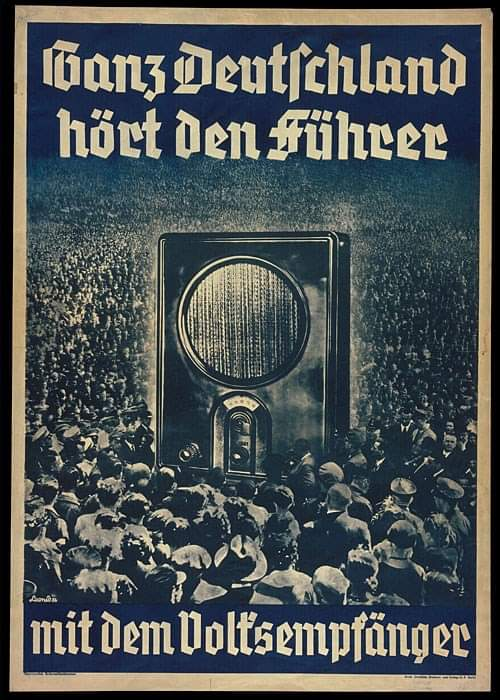
\includegraphics[width=0.4\textwidth,height=\textheight]{vis/volksempfanger.jpg}
\end{frame}

\hypertarget{literature-and-theory}{%
\section{Literature and Theory}\label{literature-and-theory}}

\begin{frame}[allowframebreaks]{Media effects - maximal or minimal?}
\protect\hypertarget{media-effects---maximal-or-minimal}{}
Maximal paradigm also follows from classic work:

\begin{itemize}
\tightlist
\item
  attitude instability (Converse 1962; Zaller 1992)
\item
  agenda-setting (McCombs and Shaw 1972)
\item
  framing (Nelson, Clawson, and Oxley 1997)
\end{itemize}

\framebreak

Minimal effects assumption with increasing media diversity (Bennett and
Iyengar 2008):

\begin{itemize}
\tightlist
\item
  media environment more polarised and more diverse,
\item
  viewers more likely to reject news conflicting with their views,
\item
  viewers can opt for other sources.
\end{itemize}

\(\rightarrow\) strong effects unlikely
\end{frame}

\begin{frame}[allowframebreaks]{Empirical evidence}
\protect\hypertarget{empirical-evidence}{}
\begin{block}{Evidence for large effects}
\protect\hypertarget{evidence-for-large-effects}{}
\begin{itemize}
\tightlist
\item
  Framing effects found in experimental data (Busby, Flynn, and Druckman
  2019; Leeper and Slothuus 2020).
\item
  Newspaper slant affects attitudes (Foos and Bischof 2020).
\item
  Salience and tonality of migration news affects attitudes (Boomgaarden
  and Vliegenthart 2009).
\end{itemize}
\end{block}

\begin{block}{Evidence for no/weak effects}
\protect\hypertarget{evidence-for-noweak-effects}{}
\begin{itemize}
\tightlist
\item
  Newspaper slant has no effect on attitudes (Gentzkow, Shapiro, and
  Sinkinson 2011; Guess et al. 2021; Štětka, Mihelj, and Tóth 2020).
\item
  Newspaper takeovers have no effect on attitudes (Durante and Knight
  2012; Spirig 2020).
\end{itemize}
\end{block}
\end{frame}

\begin{frame}{Synthesis}
\protect\hypertarget{synthesis}{}
\textbf{When} can we expect strong media effects?

\begin{itemize}
\tightlist
\item
  Many current approaches test media effects of different outlets
  (Gentzkow, Shapiro, and Sinkinson 2011; Guess et al. 2021).
\item
  However, \textbf{news consumers discount bias and take cues from
  outlets}.

  \begin{itemize}
  \tightlist
  \item
    Baum and Gussin (2008) show that consumers take heuristics about
    content bias from outlet brands.
  \item
    Chiang and Knight (2011) show that outlet bias moderates the effect
    of candidate endorsements.
  \end{itemize}
\end{itemize}

\(\rightarrow\) \textbf{within-outlet changes} in content most likely
cases to observe media effects.
\end{frame}

\begin{frame}[allowframebreaks]{Emphasis framing}
\protect\hypertarget{emphasis-framing}{}
\textbf{What kind of changes should matter?}

\begin{itemize}
\tightlist
\item
  I draw on literature on

  \begin{itemize}
  \tightlist
  \item
    the \textbf{value-expectancy} framework (Ajzen and Fishbein 2000).
  \item
    and \textbf{emphasis framing} (Leeper and Slothuus 2020; Nelson,
    Clawson, and Oxley 1997).
  \end{itemize}
\item
  Argues that issue attitudes are a product of \textbf{associated
  considerations}.
\end{itemize}

\framebreak

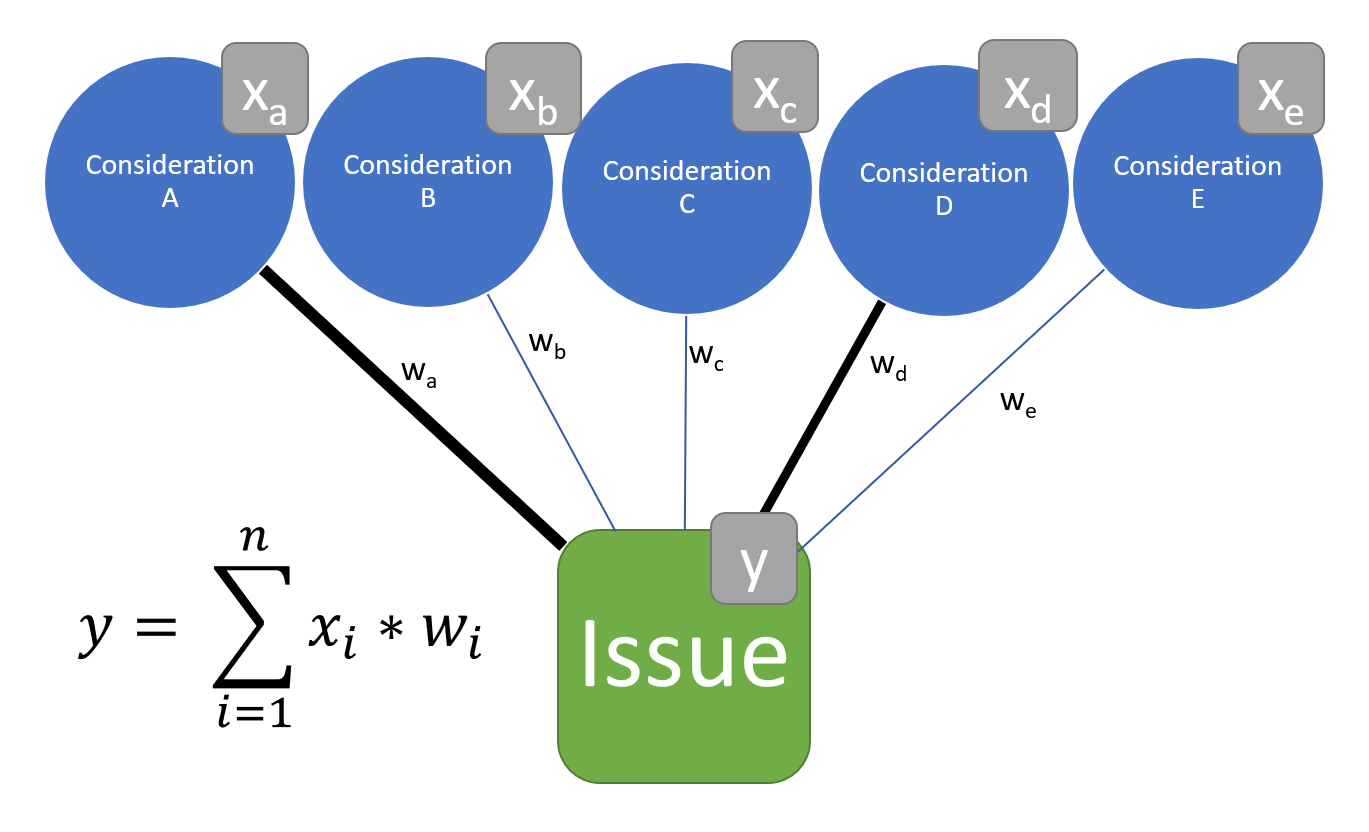
\includegraphics{vis/CognitiveStorage.png}
\end{frame}

\hypertarget{empirical-strategy}{%
\section{Empirical strategy}\label{empirical-strategy}}

\begin{frame}{The case: Germany 2017}
\protect\hypertarget{the-case-germany-2017}{}
\begin{itemize}
\tightlist
\item
  First election after 2015 refugee movements.
\item
  Radical-right challenger party enters parliament, center loses.
\item
  Migration top of the agenda.
\end{itemize}

\(\rightarrow\) constantly strong attention to migration,

\(\rightarrow\) good case to study effects of framing.
\end{frame}

\begin{frame}{Design}
\protect\hypertarget{design}{}
\begin{itemize}
\tightlist
\item
  Collect 2.5M articles from major German newspapers.
\item
  Classify according to migration content.
\item
  Identify emphasis frames.
\item
  Correlate changes in framing with changes in attitudes.
\end{itemize}
\end{frame}

\begin{frame}[allowframebreaks]{Issue attitudes and news consumption}
\protect\hypertarget{issue-attitudes-and-news-consumption}{}
\begin{itemize}
\tightlist
\item
  Panel data from the German Longitudinal Election Study (GLES 2019).
\item
  Contains questions on news consumption and immigration and integration
  attitudes.
\item
  6 waves in 2017, containing both items.
\item
  Immigration attitude measured on a 7-point Likert scale:

  \begin{itemize}
  \tightlist
  \item
    ``\emph{Immigration should be made easier (-3) or restricted (3)}.''
  \end{itemize}
\end{itemize}
\end{frame}

\begin{frame}[allowframebreaks]{Migration content}
\protect\hypertarget{migration-content}{}
\begin{itemize}
\tightlist
\item
  Pre-assign likelihoods for migration content using extended migration
  dictionary.
\item
  Draw stratified sample of 1,800 articles, hand-code.
\item
  Fine-tune German BERT deep-learning classifier.
\item
  Performs very well: F1: 0.94, recall: 0.93, precision: 0.95.
\item
  13.5k out of 400k articles in 2017 about migration (3.5\%)
\end{itemize}

\framebreak

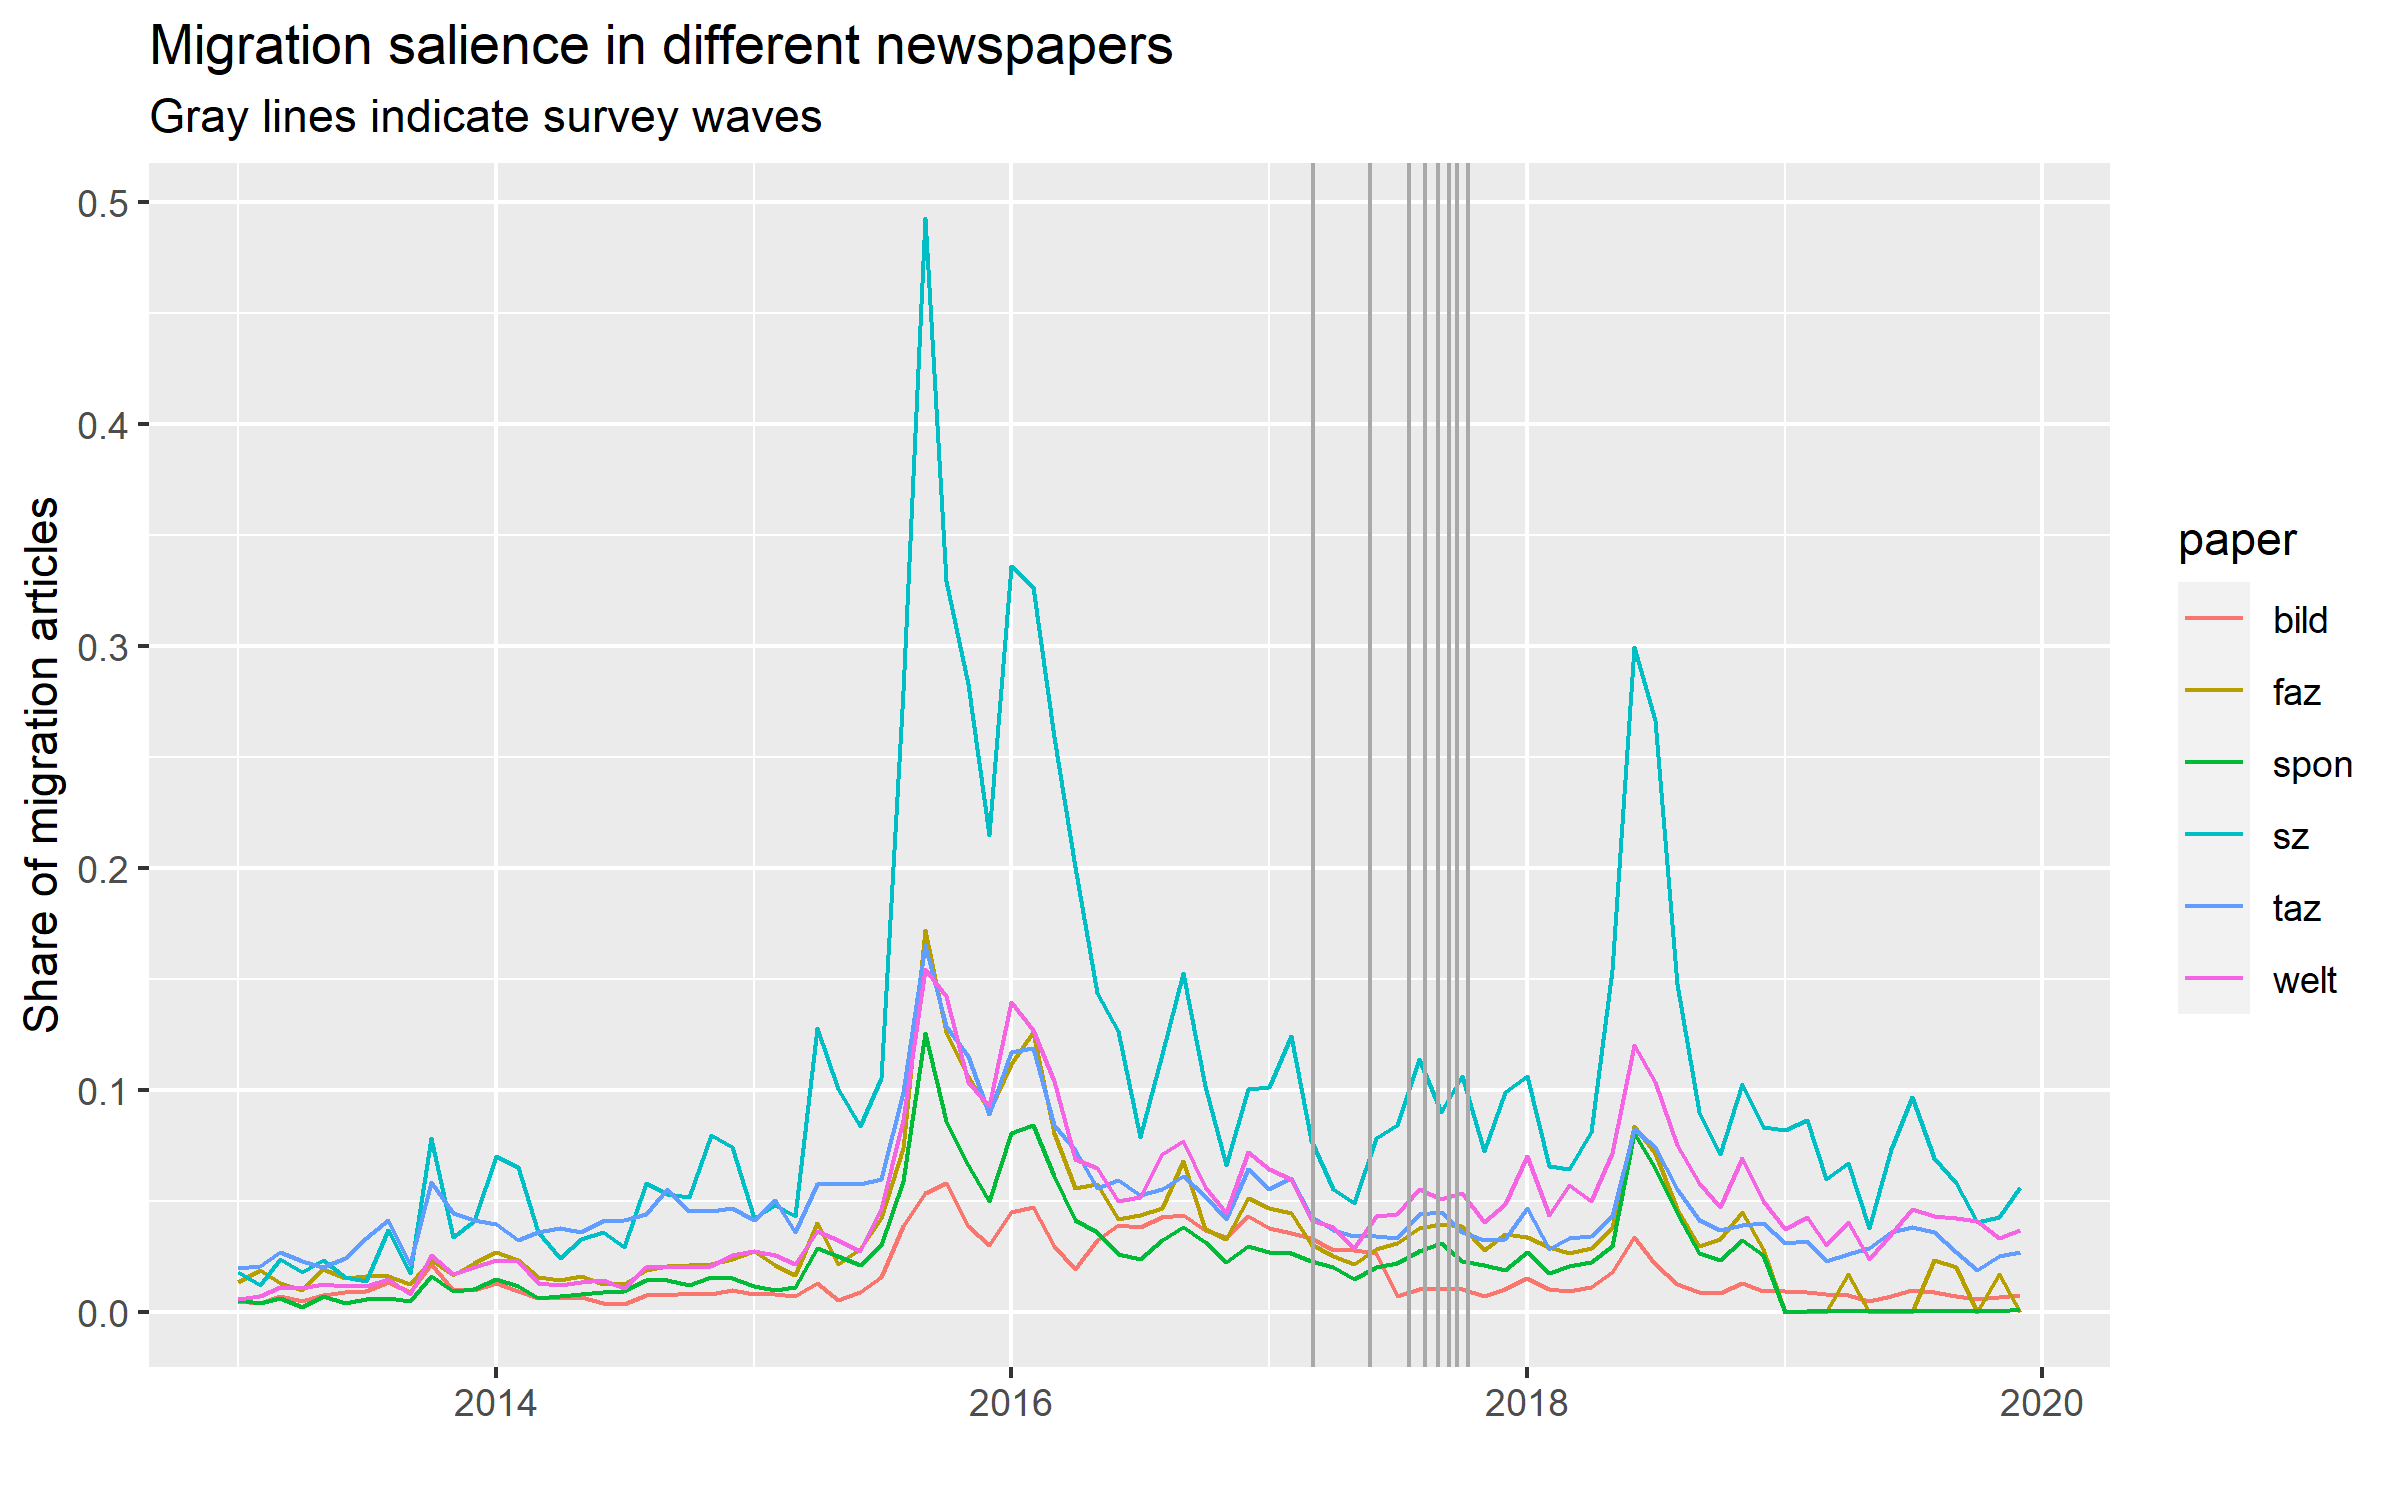
\includegraphics{vis/salience_papers.png}
\end{frame}

\begin{frame}[allowframebreaks]{Migration framing}
\protect\hypertarget{migration-framing}{}
\begin{itemize}
\tightlist
\item
  Estimate 60-topic structural topic model (Roberts et al. 2014), using
  date and paper as covariates.
\item
  Annotate.
\item
  Select relevant frames with clear expectations regarding attitudinal
  effects.
\end{itemize}

\framebreak

\textbf{Topics}:

\begin{itemize}
\tightlist
\item
  Capital crime (sexual assault/rape/murder) committed by refugees,
\item
  illegal entry and petty crime,
\item
  refugee numbers,
\item
  labour market needs for and job market integration of refugees,
\item
  deportations,
\item
  internment camps (e.g.~Moria),
\item
  drownings in the Mediterranean.
\end{itemize}

\framebreak

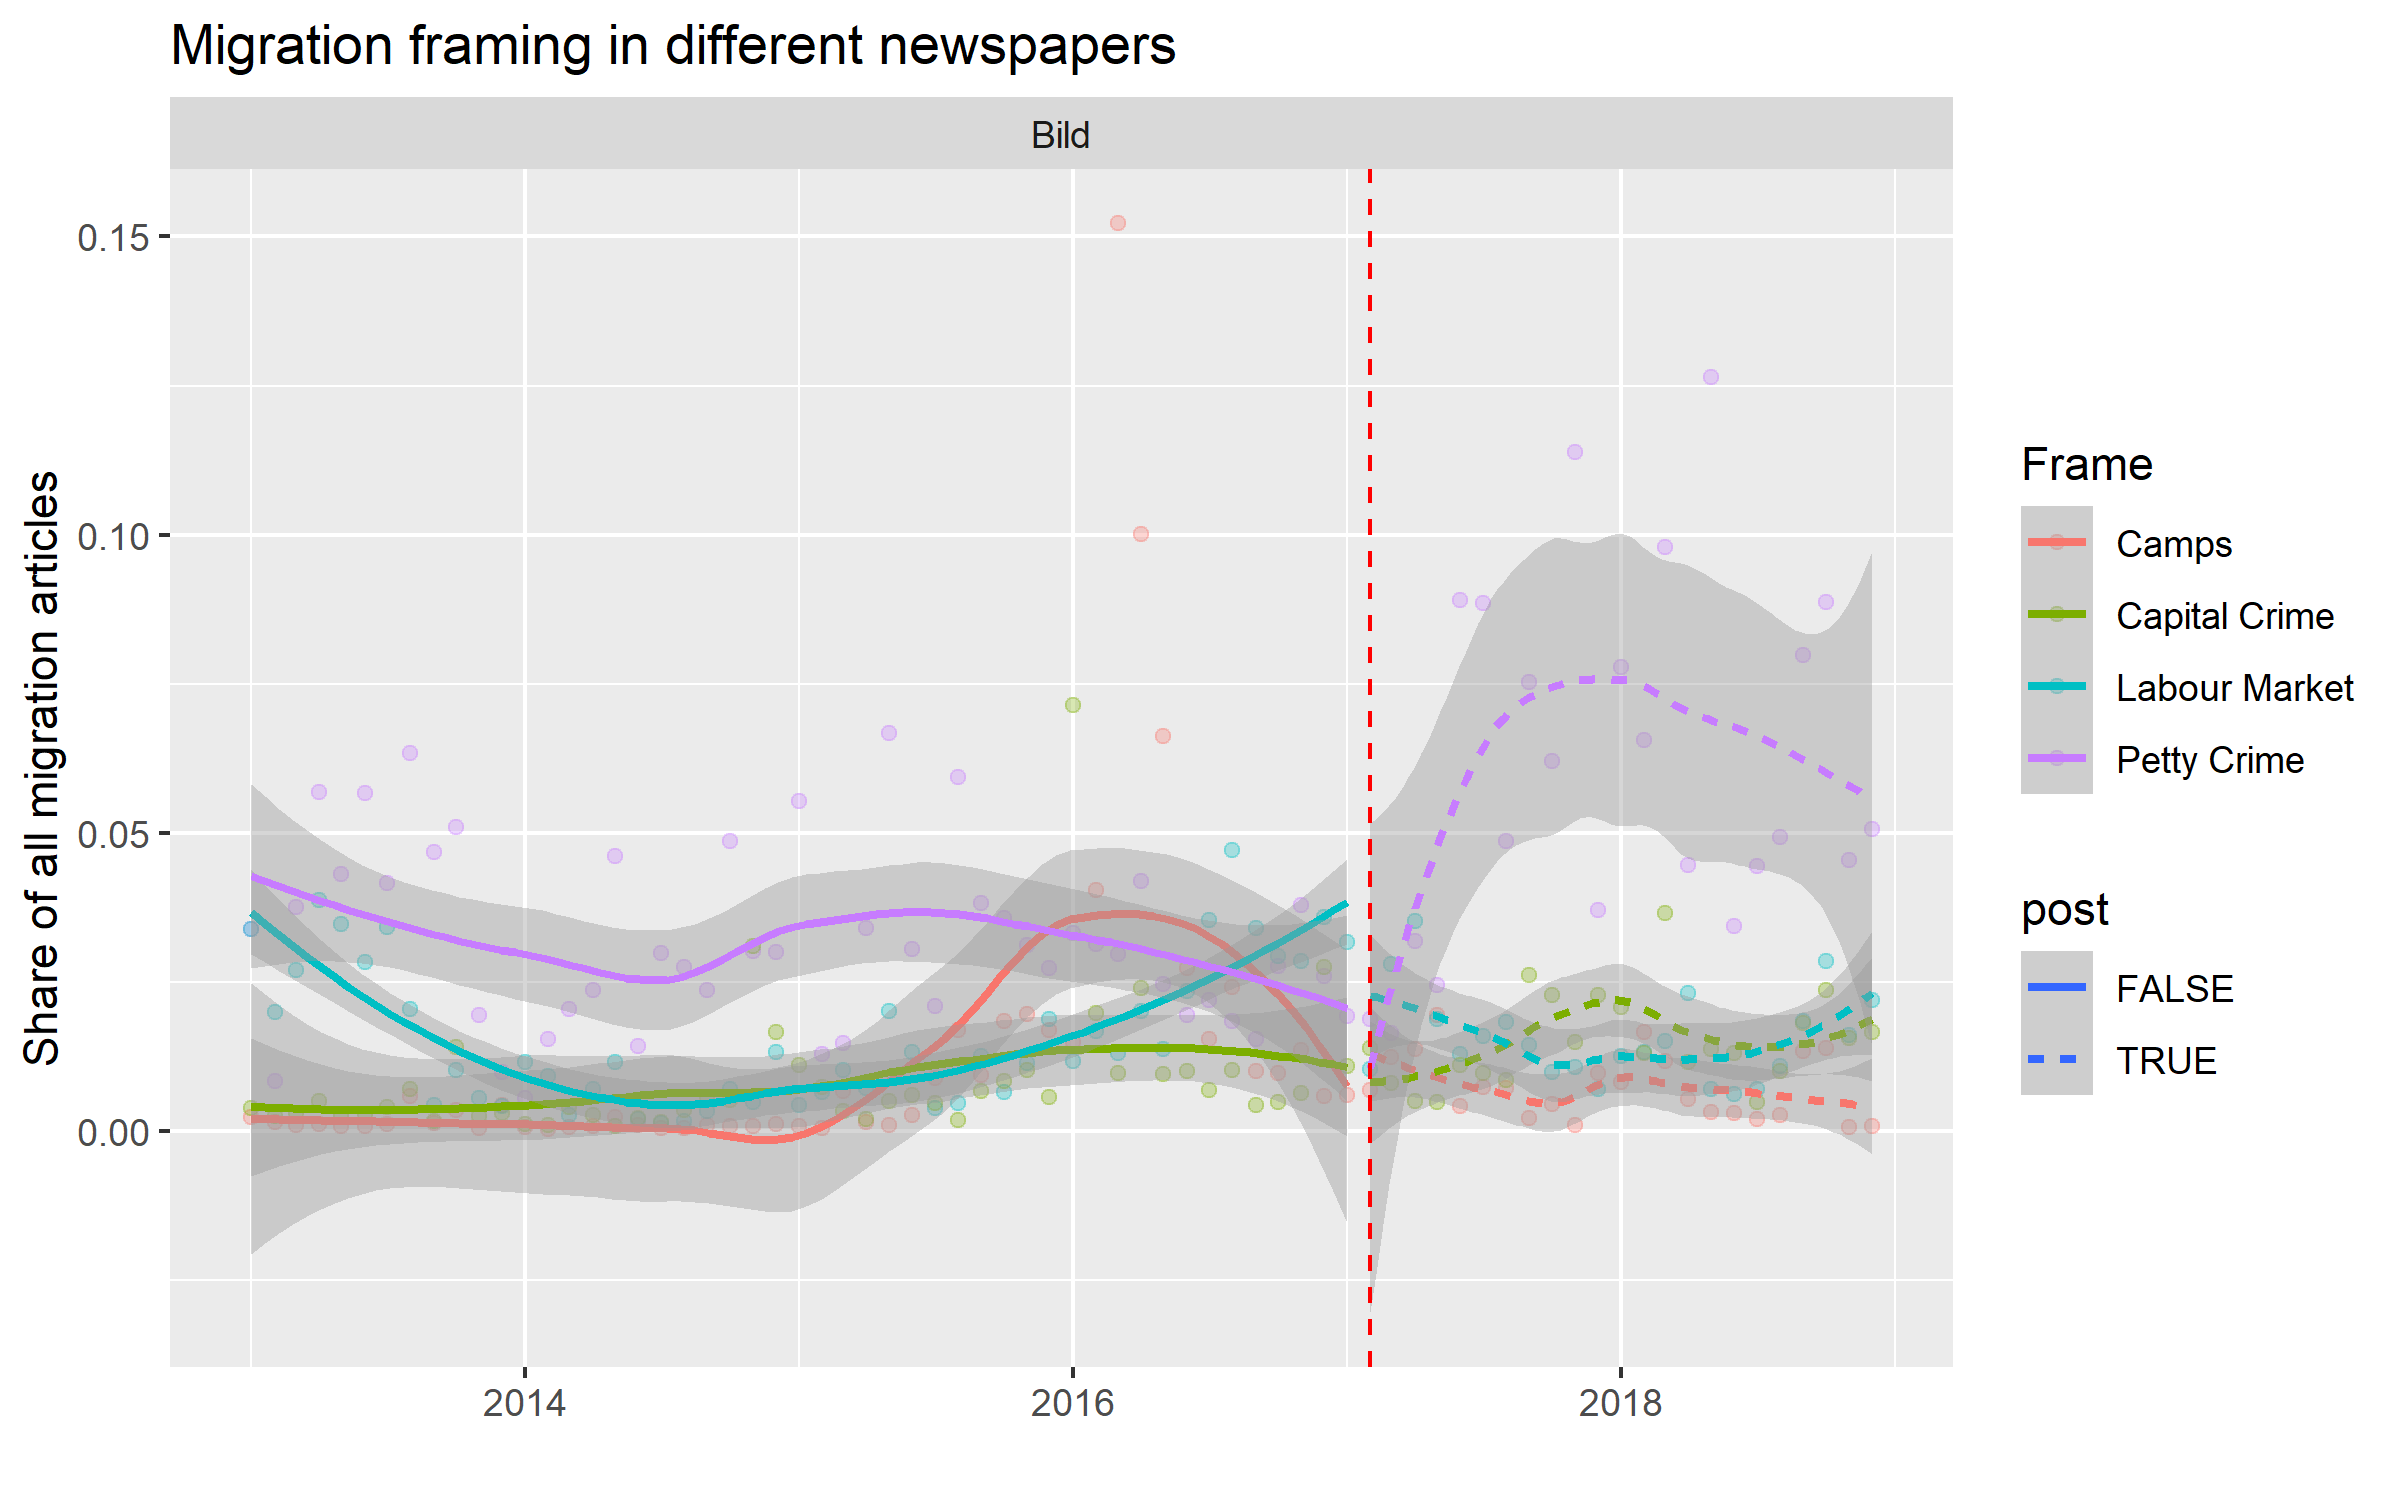
\includegraphics{vis/frames_papers_pres.png}
\end{frame}

\begin{frame}{Estimation}
\protect\hypertarget{estimation}{}
\emph{Two models}:

\begin{itemize}
\tightlist
\item
  OLS of aggregate Difference-in-Differences (DiDs).
\item
  Individual-level model with 2-way fixed effects.
\end{itemize}
\end{frame}

\begin{frame}[allowframebreaks]{DiD-model}
\protect\hypertarget{did-model}{}
\[y = \beta_1*W + \beta_2*R + \beta_3*W*R\]

\centering

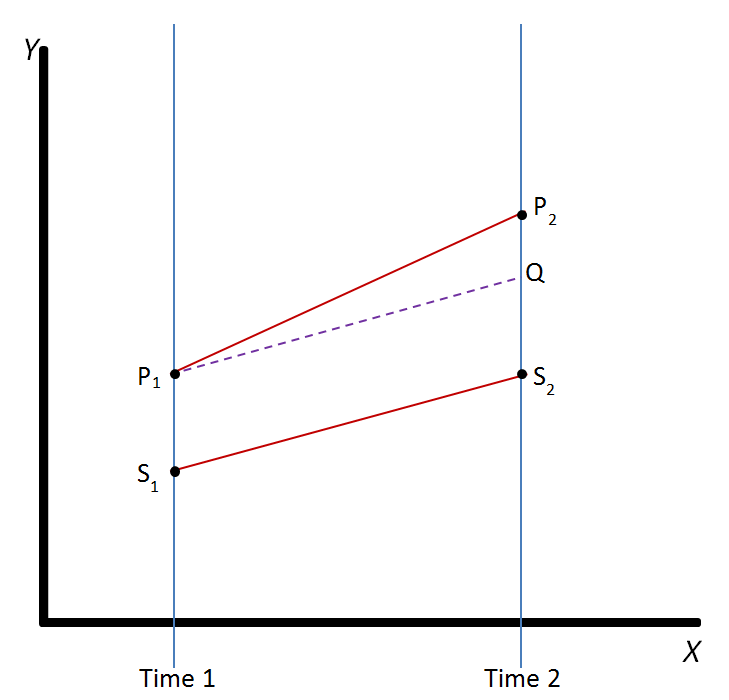
\includegraphics[width=0.5\textwidth,height=\textheight]{vis/Illustration_of_Difference_in_Differences.png}

\framebreak

\begin{itemize}
\tightlist
\item
  Estimate change in newspaper framing and attitudes among readers from
  one wave to another, controlling for shifts in other newspapers/reader
  groups.
\item
  Regress opinion shift among readership on shift in newspaper attention
  to different frames.
\item
  Better identified (exact change \emph{beyond} general trend),
\item
  but framing not individually matched.
\end{itemize}
\end{frame}

\begin{frame}[allowframebreaks]{2-way FE model}
\protect\hypertarget{way-fe-model}{}
\begin{itemize}
\tightlist
\item
  Individual estimate of frame attention for each respondent, according
  to newspaper read.
\item
  Regress opinion on exposure to each frame,
\item
  controlling for wave and individual fixed-effects.
\end{itemize}

\framebreak

\begin{itemize}
\tightlist
\item
  Individual estimates,
\item
  but explains \emph{all} variation beyond

  \begin{itemize}
  \tightlist
  \item
    time-independent individual factors and
  \item
    general trends across time,
  \item
    including random individual deviations.
  \end{itemize}
\end{itemize}
\end{frame}

\hypertarget{preliminary-results}{%
\section{Preliminary results}\label{preliminary-results}}

\begin{frame}{Preliminary results}
Different specifications:

\begin{itemize}
\tightlist
\item
  all readers/exclusive readers of one newspaper,
\item
  different lags to measure exposure (1 day, 1 week, 1 month, half a
  year),
\item
  immigration and integration attitude as dependent variable.
\end{itemize}
\end{frame}

\begin{frame}[allowframebreaks]{Difference-in-Difference model}
\protect\hypertarget{difference-in-difference-model}{}
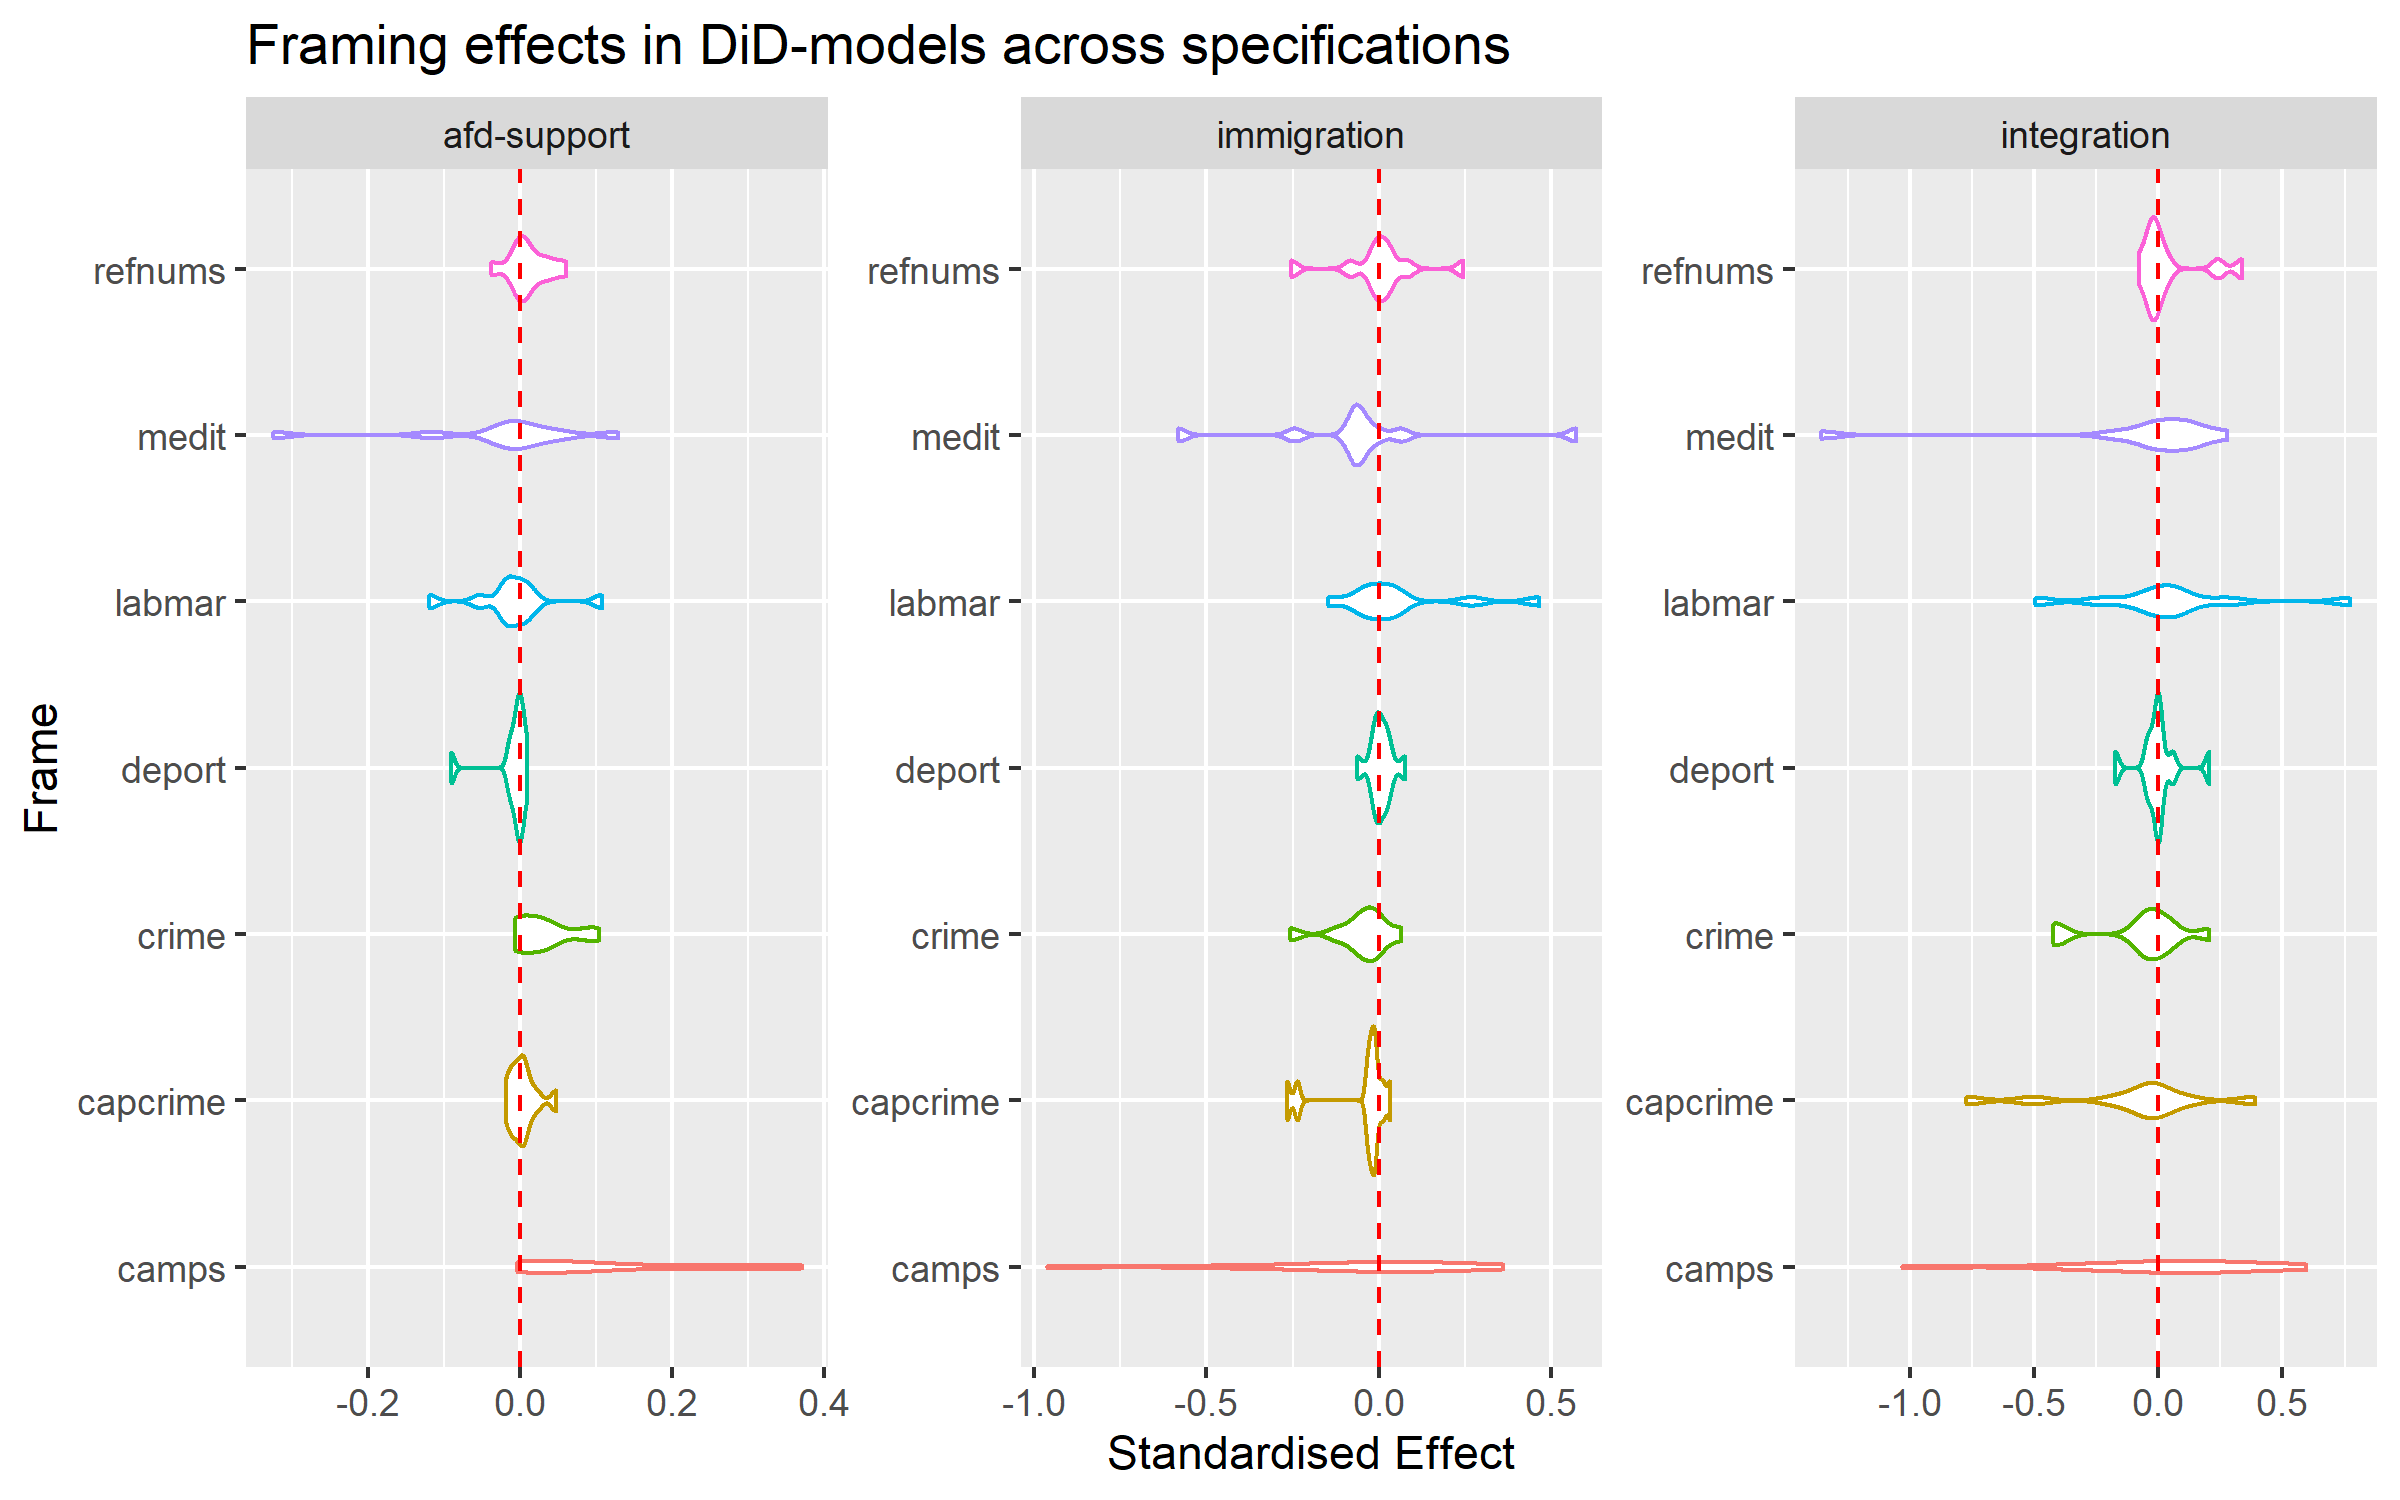
\includegraphics{vis/frame_effects_did.png}
\end{frame}

\begin{frame}{Fixed-effect model}
\protect\hypertarget{fixed-effect-model}{}
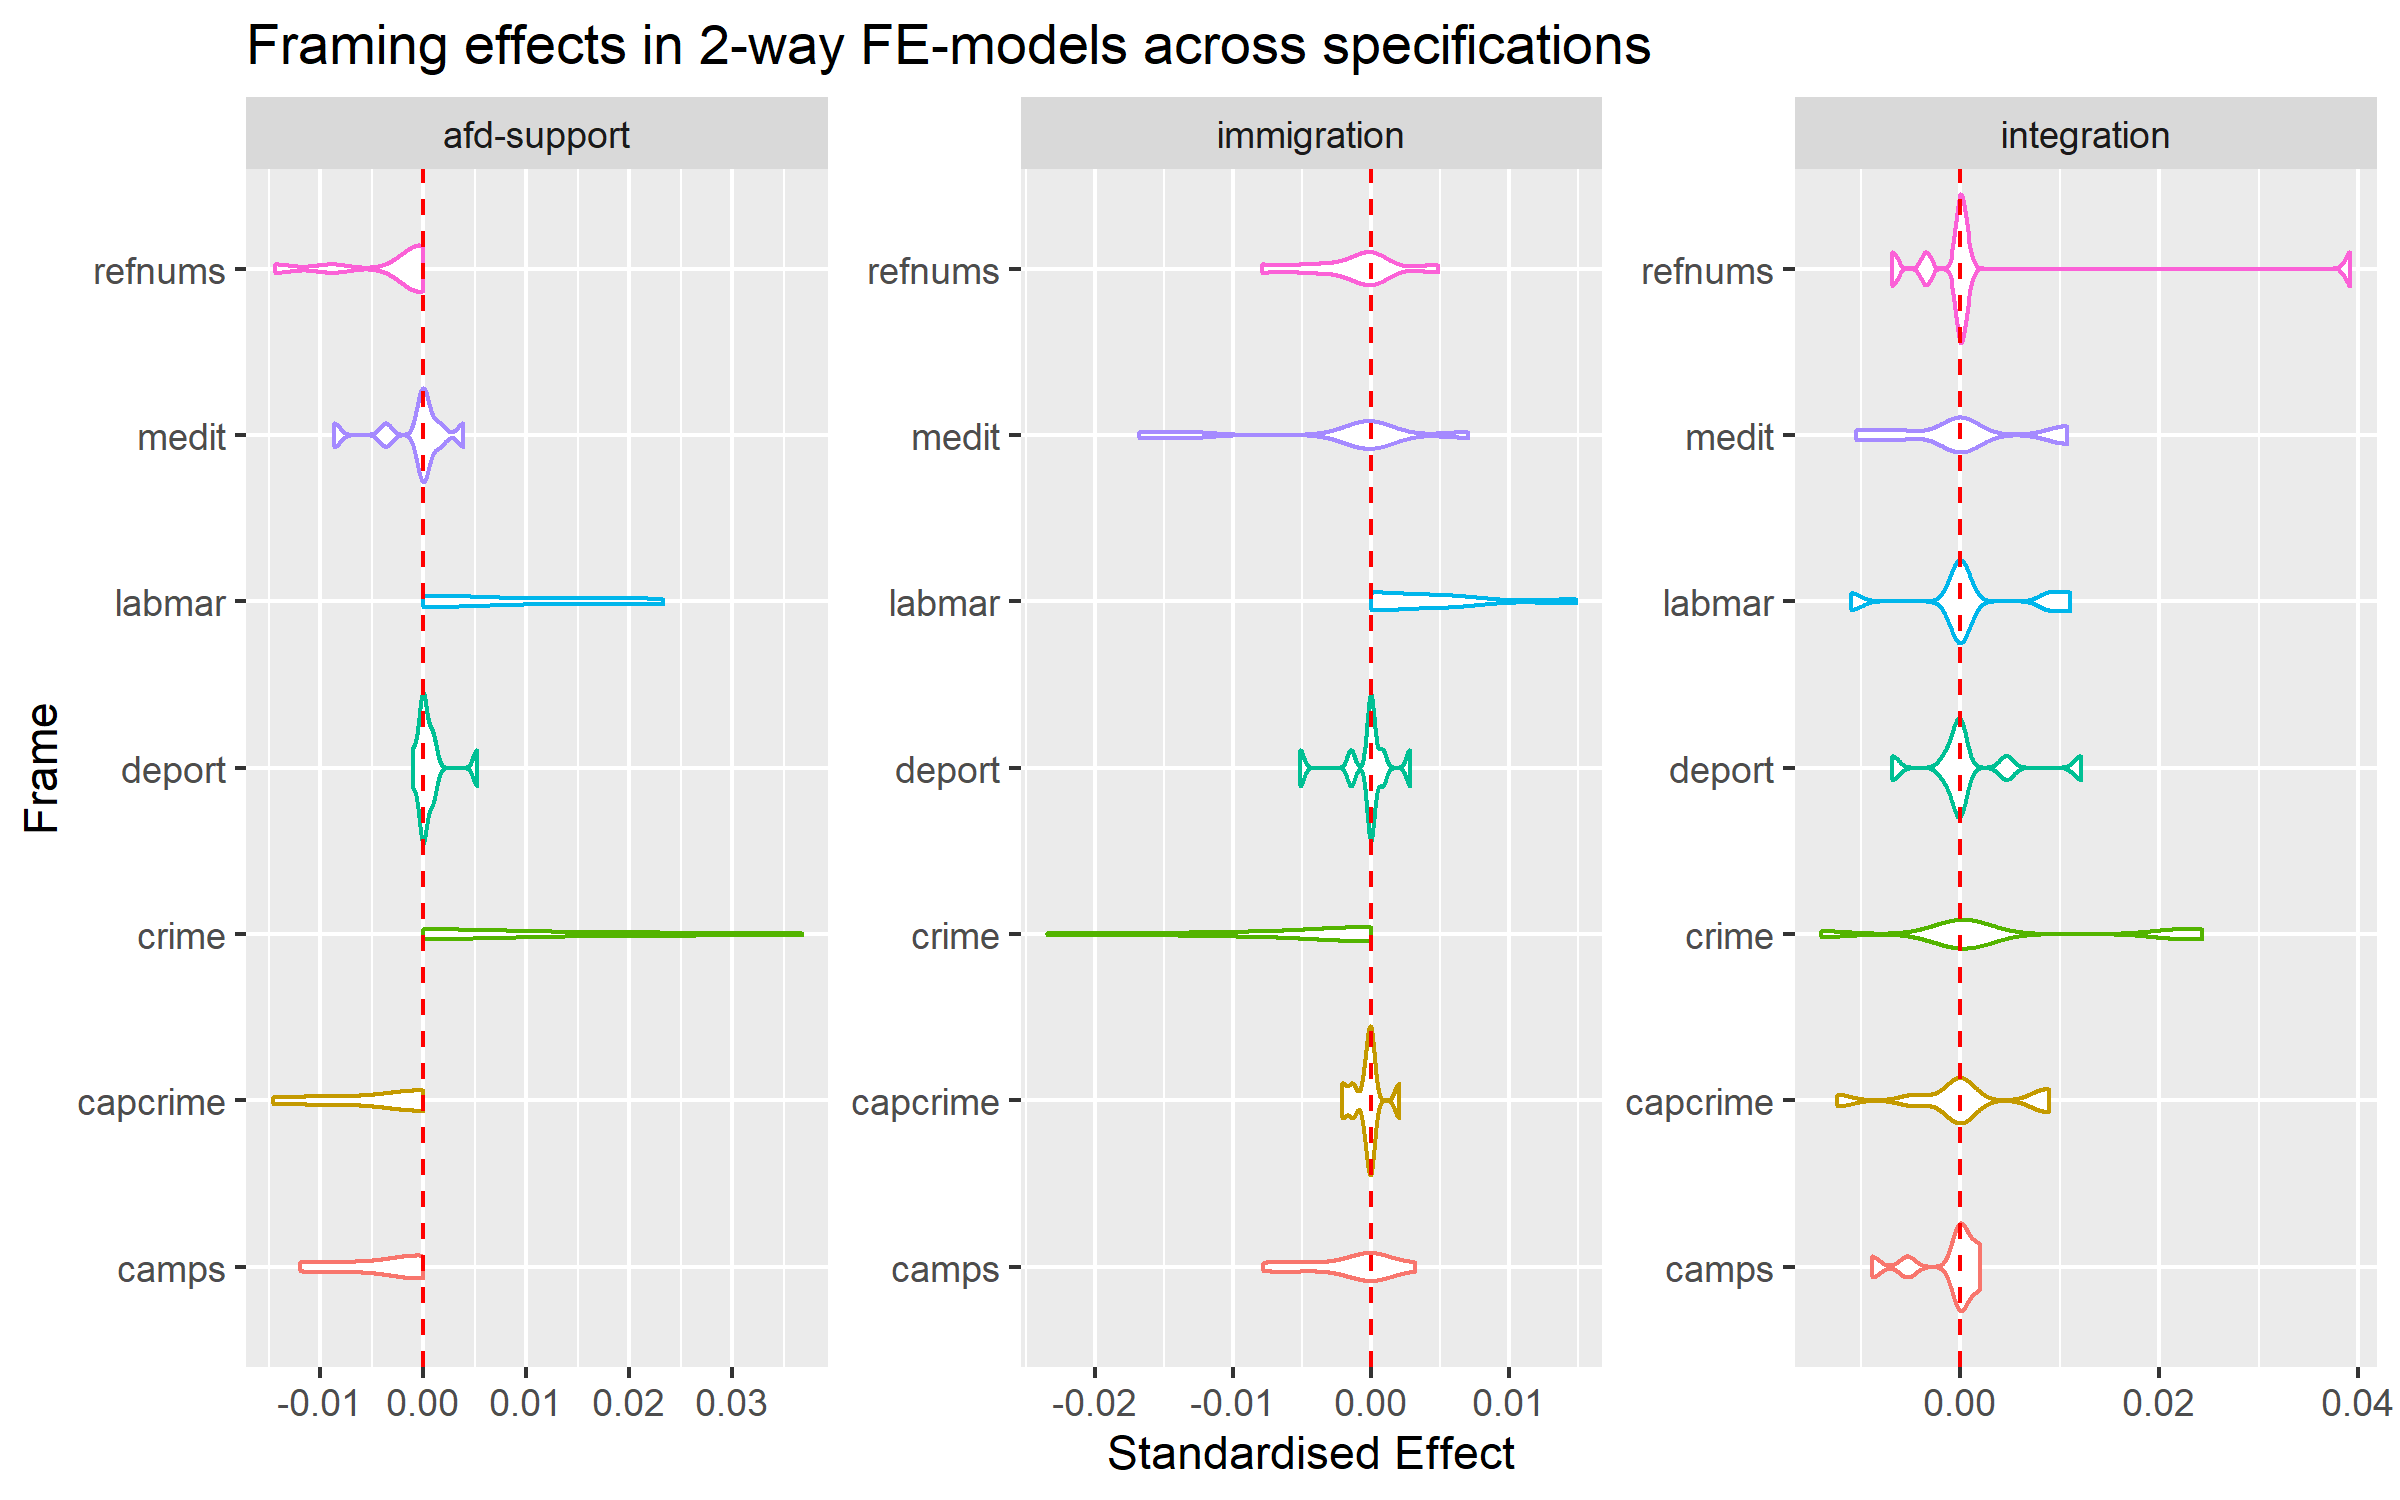
\includegraphics{vis/frame_effects_fe.png}
\end{frame}

\begin{frame}{Preliminary conclusion}
\protect\hypertarget{preliminary-conclusion}{}
\begin{itemize}
\tightlist
\item
  No effects of media framing even in most-likely case.
\item
  \emph{However}, many possible explanations:

  \begin{itemize}
  \tightlist
  \item
    Measurement issues,
  \item
    Issue-sorting in 2015, subsequent ``digging in,''
  \item
    too little variation in dependent.
  \end{itemize}
\end{itemize}

\(\rightarrow\) further work necessary\ldots{}
\end{frame}

\begin{frame}{Further hypotheses}
\protect\hypertarget{further-hypotheses}{}
\begin{itemize}
\tightlist
\item
  Motivated reasoning and polarisation (Taber and Lodge 2006).
\item
  Readers respond by changing outlet (Arceneaux and Johnson 2013).
\item
  Mobilisation, not attitudinal change (Gentzkow, Shapiro, and Sinkinson
  2011; Štětka, Mihelj, and Tóth 2020).
\end{itemize}
\end{frame}

\begin{frame}{To-do's up next}
\protect\hypertarget{to-dos-up-next}{}
\begin{itemize}
\tightlist
\item
  Clump frames together for holistic picture.
\item
  Estimate effect on readership, attitude polarisation, and AfD-support.
\item
  Natural experiment (again)?
\end{itemize}
\end{frame}

\begin{frame}{Fin}
\protect\hypertarget{fin}{}
\centering

\emph{Thank you!}
\end{frame}

\hypertarget{appendix}{%
\section{Appendix}\label{appendix}}

\begin{frame}[allowframebreaks]{Variation dependent variable}
\protect\hypertarget{variation-dependent-variable}{}
\centering

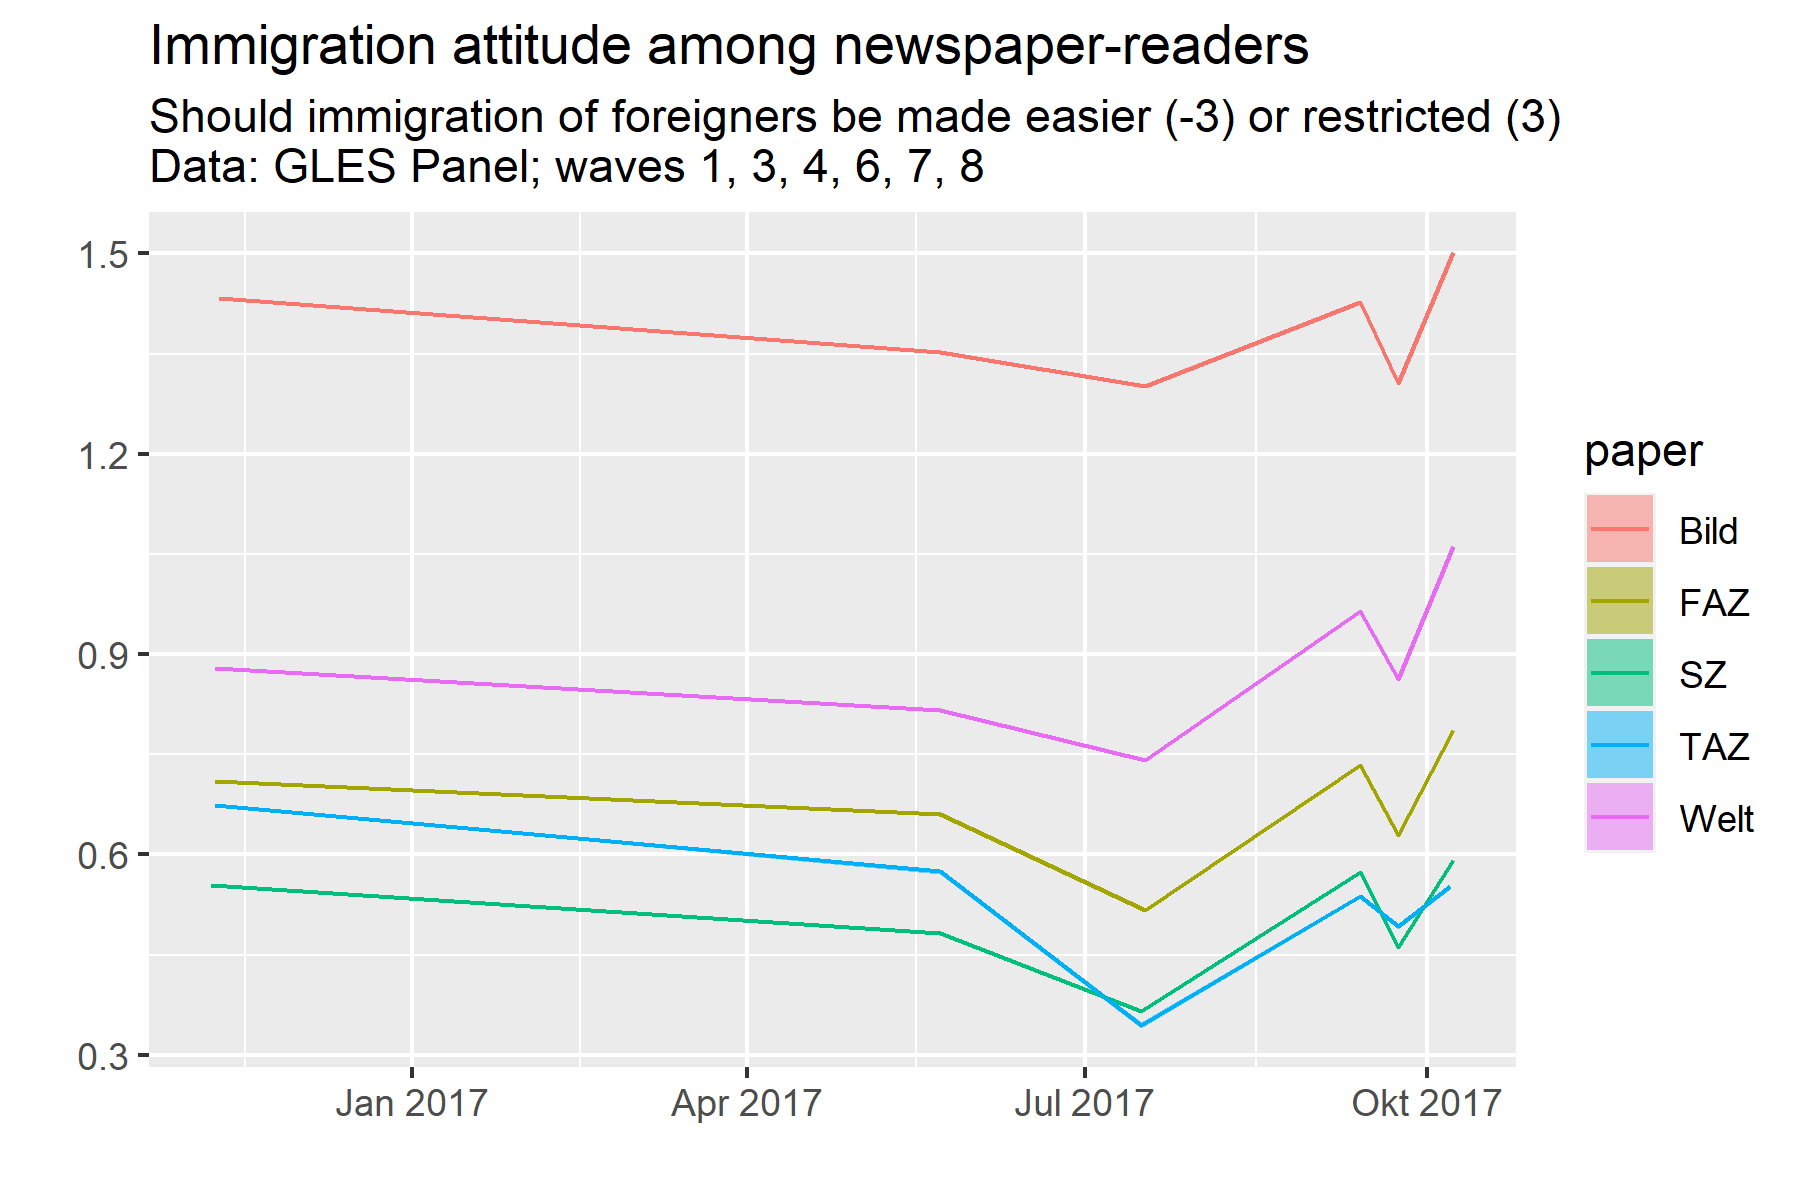
\includegraphics{vis/imm_readers_pres.png}

\framebreak

\centering

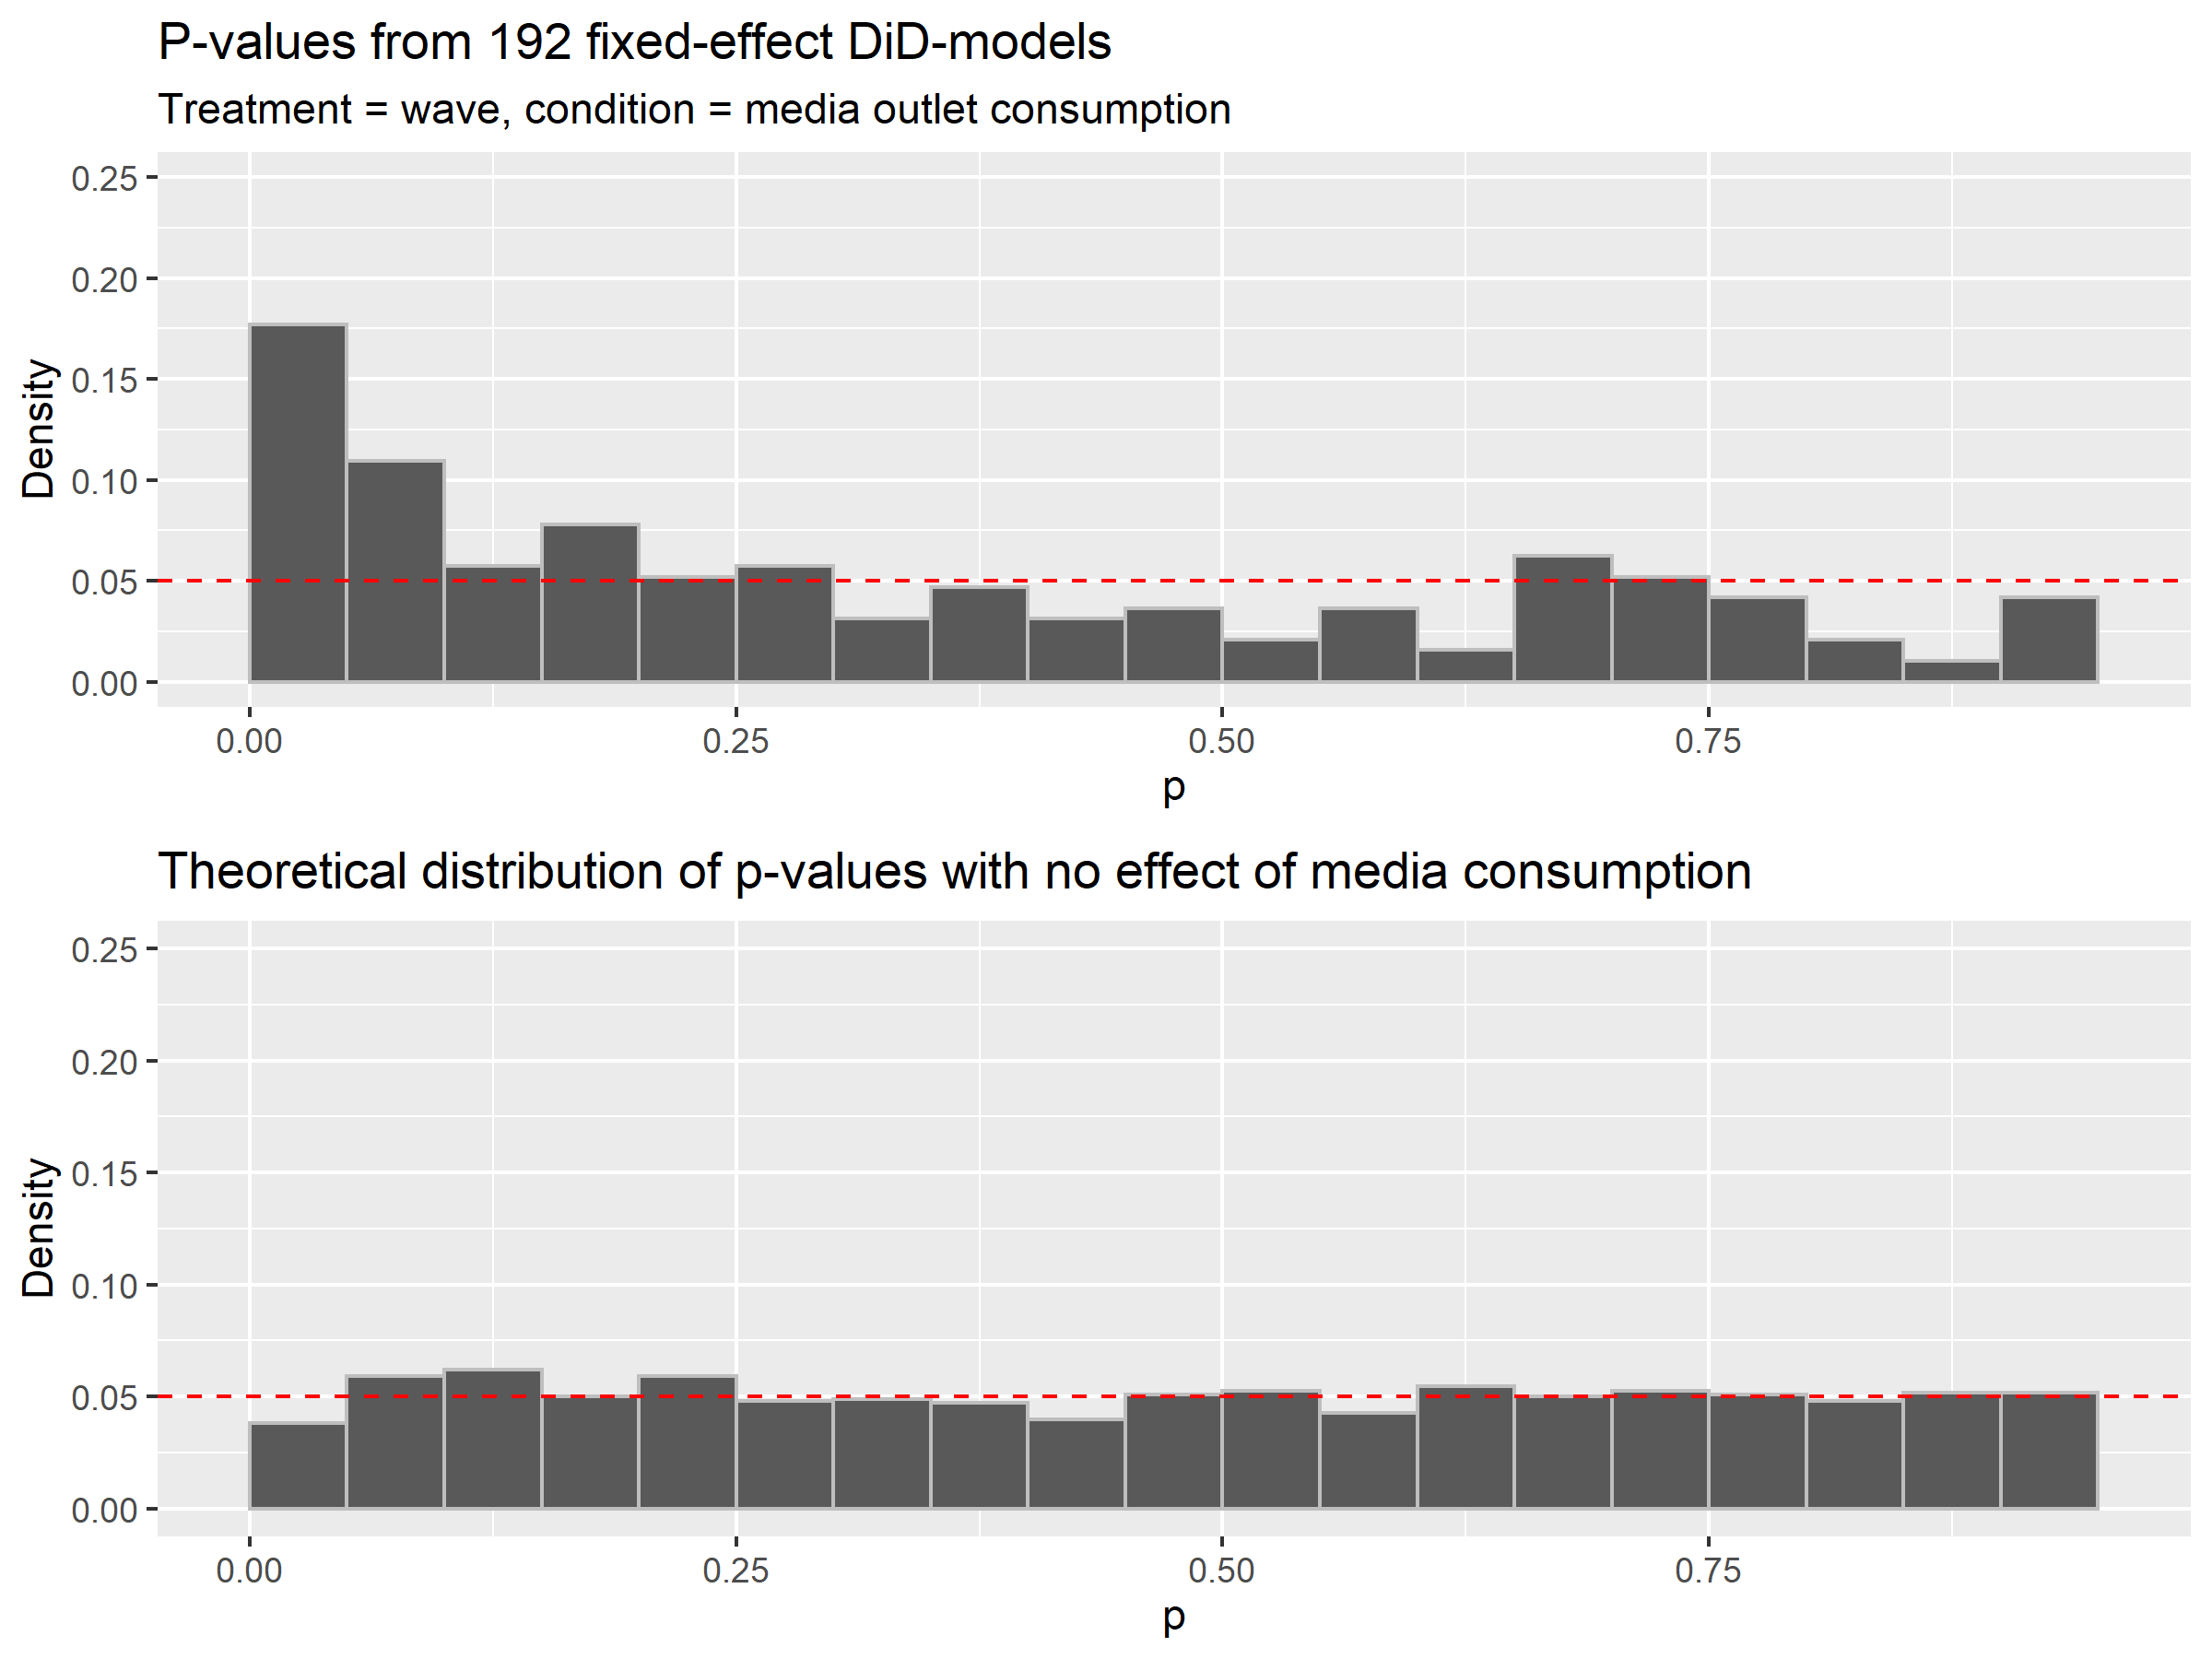
\includegraphics{vis/DiD_model_ps_immint.png}
\end{frame}

\begin{frame}[allowframebreaks]{Salience}
\protect\hypertarget{salience}{}
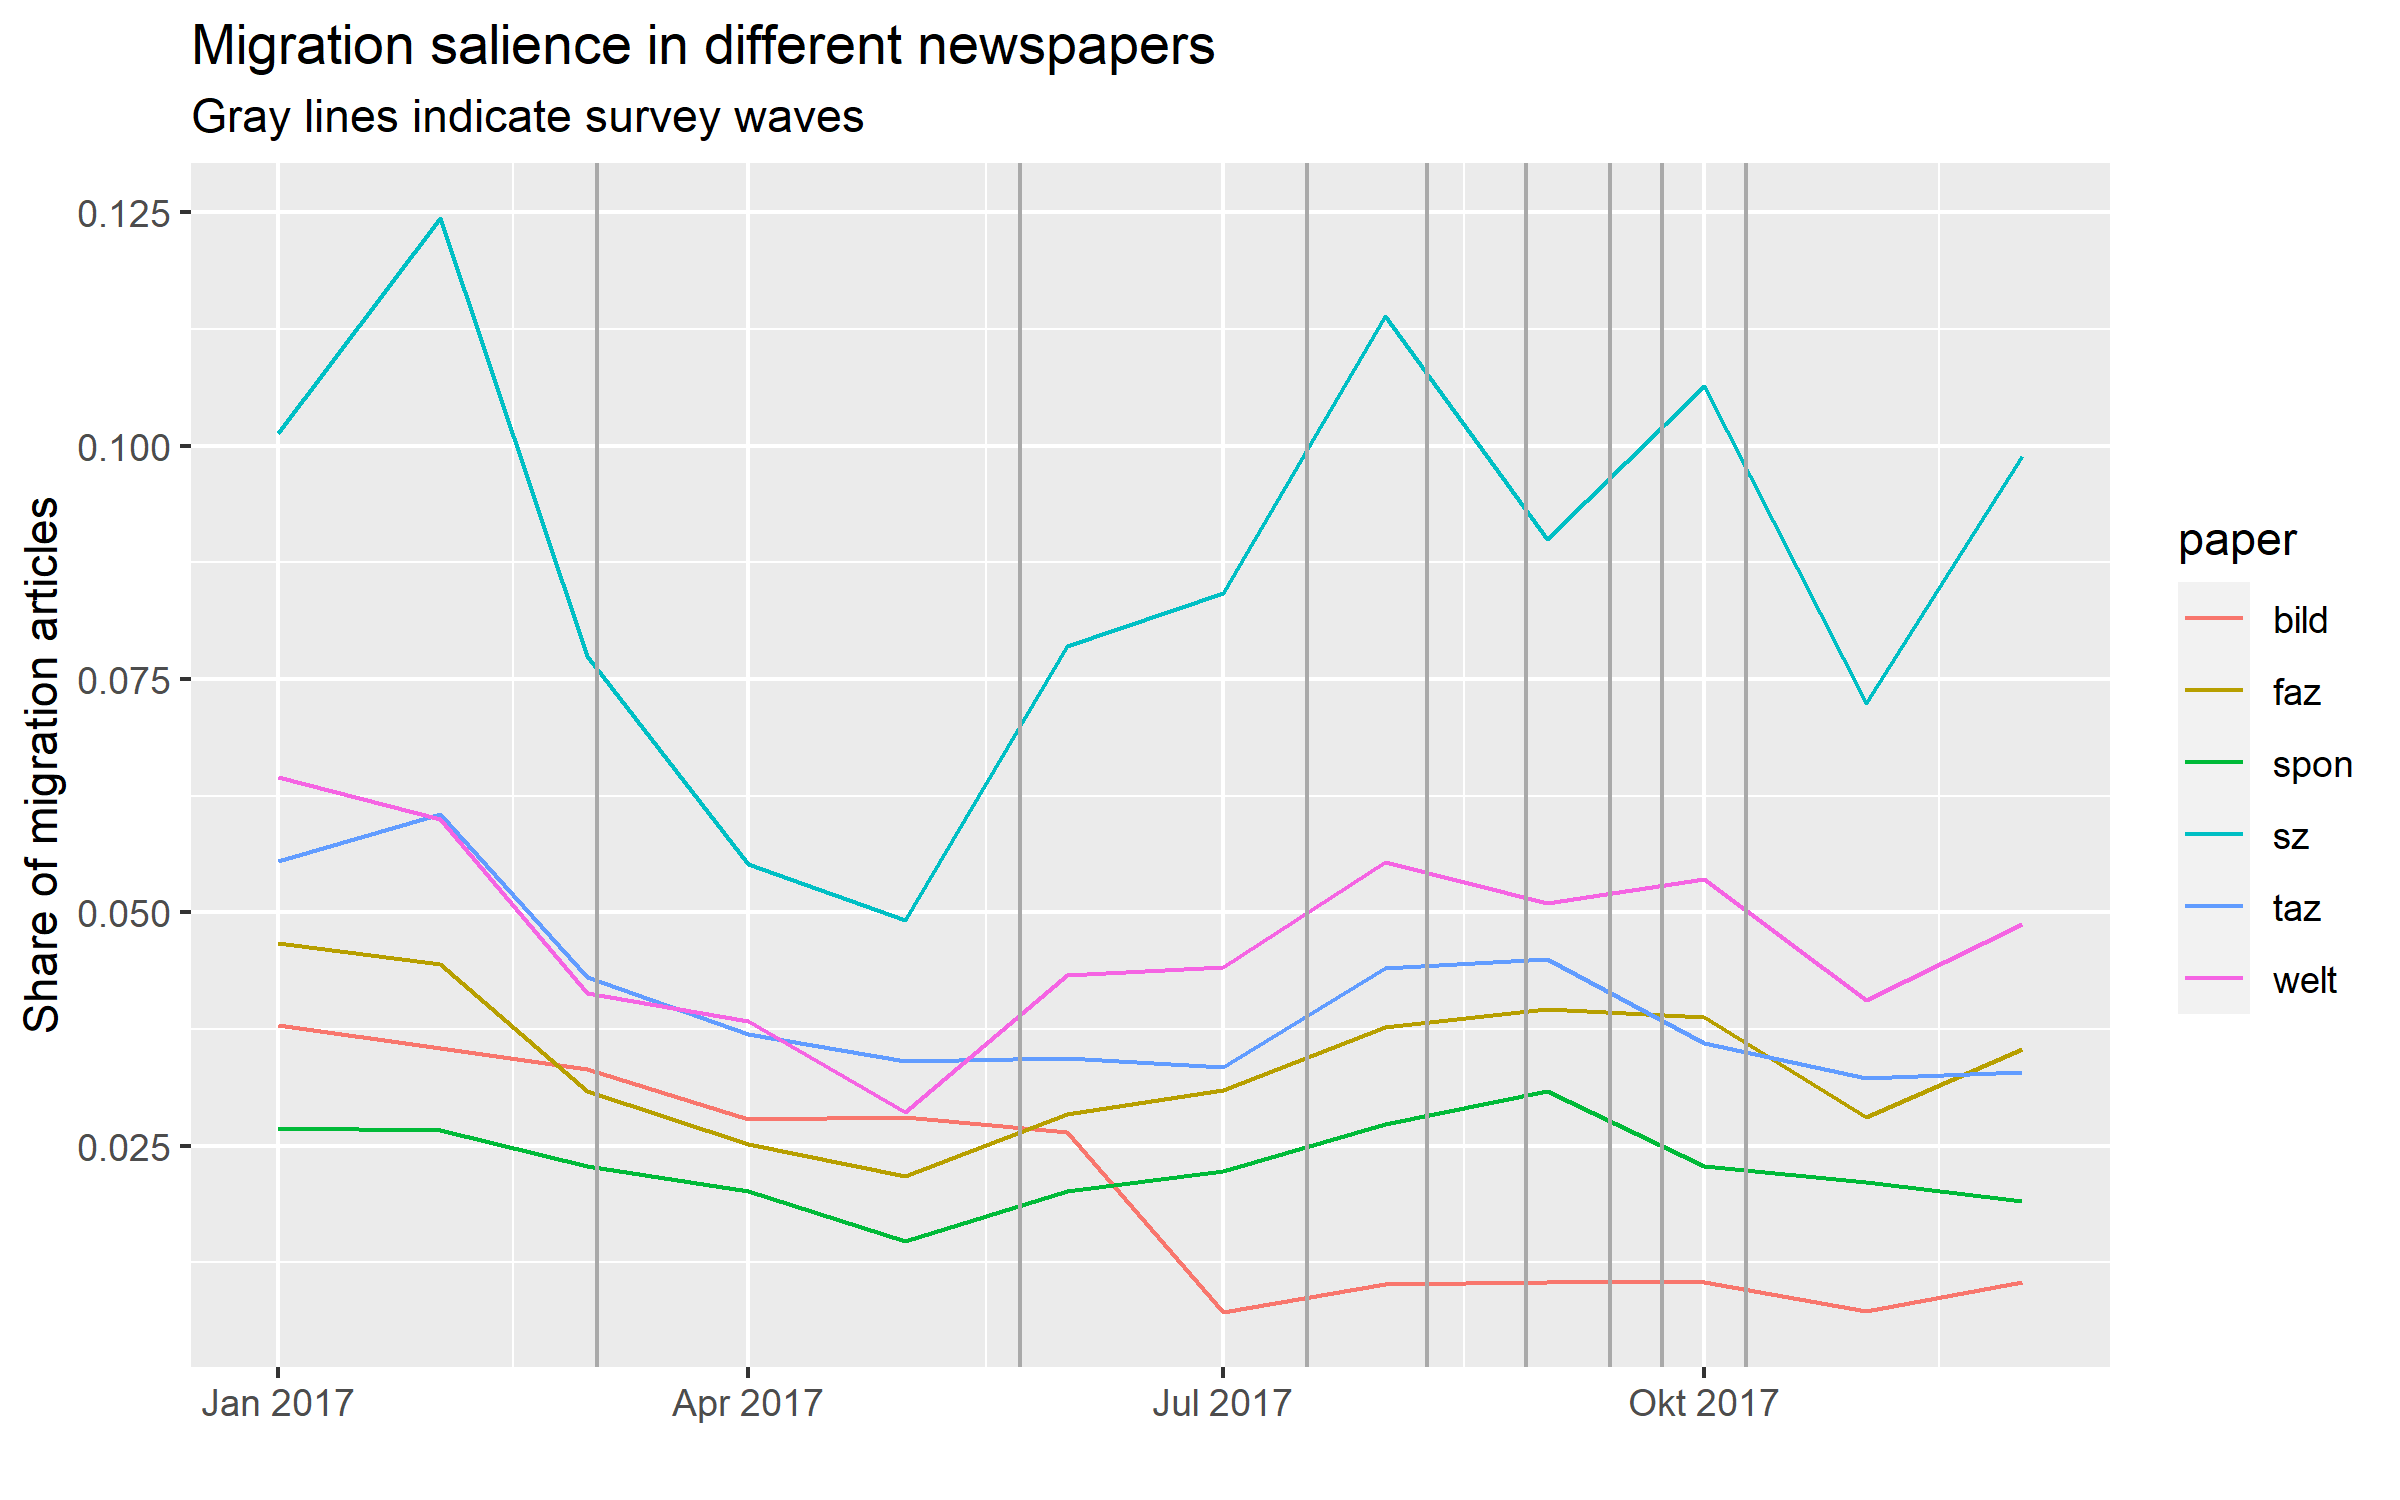
\includegraphics{vis/salience_papers_focus.png}
\end{frame}

\begin{frame}[allowframebreaks]{Framing attention}
\protect\hypertarget{framing-attention}{}
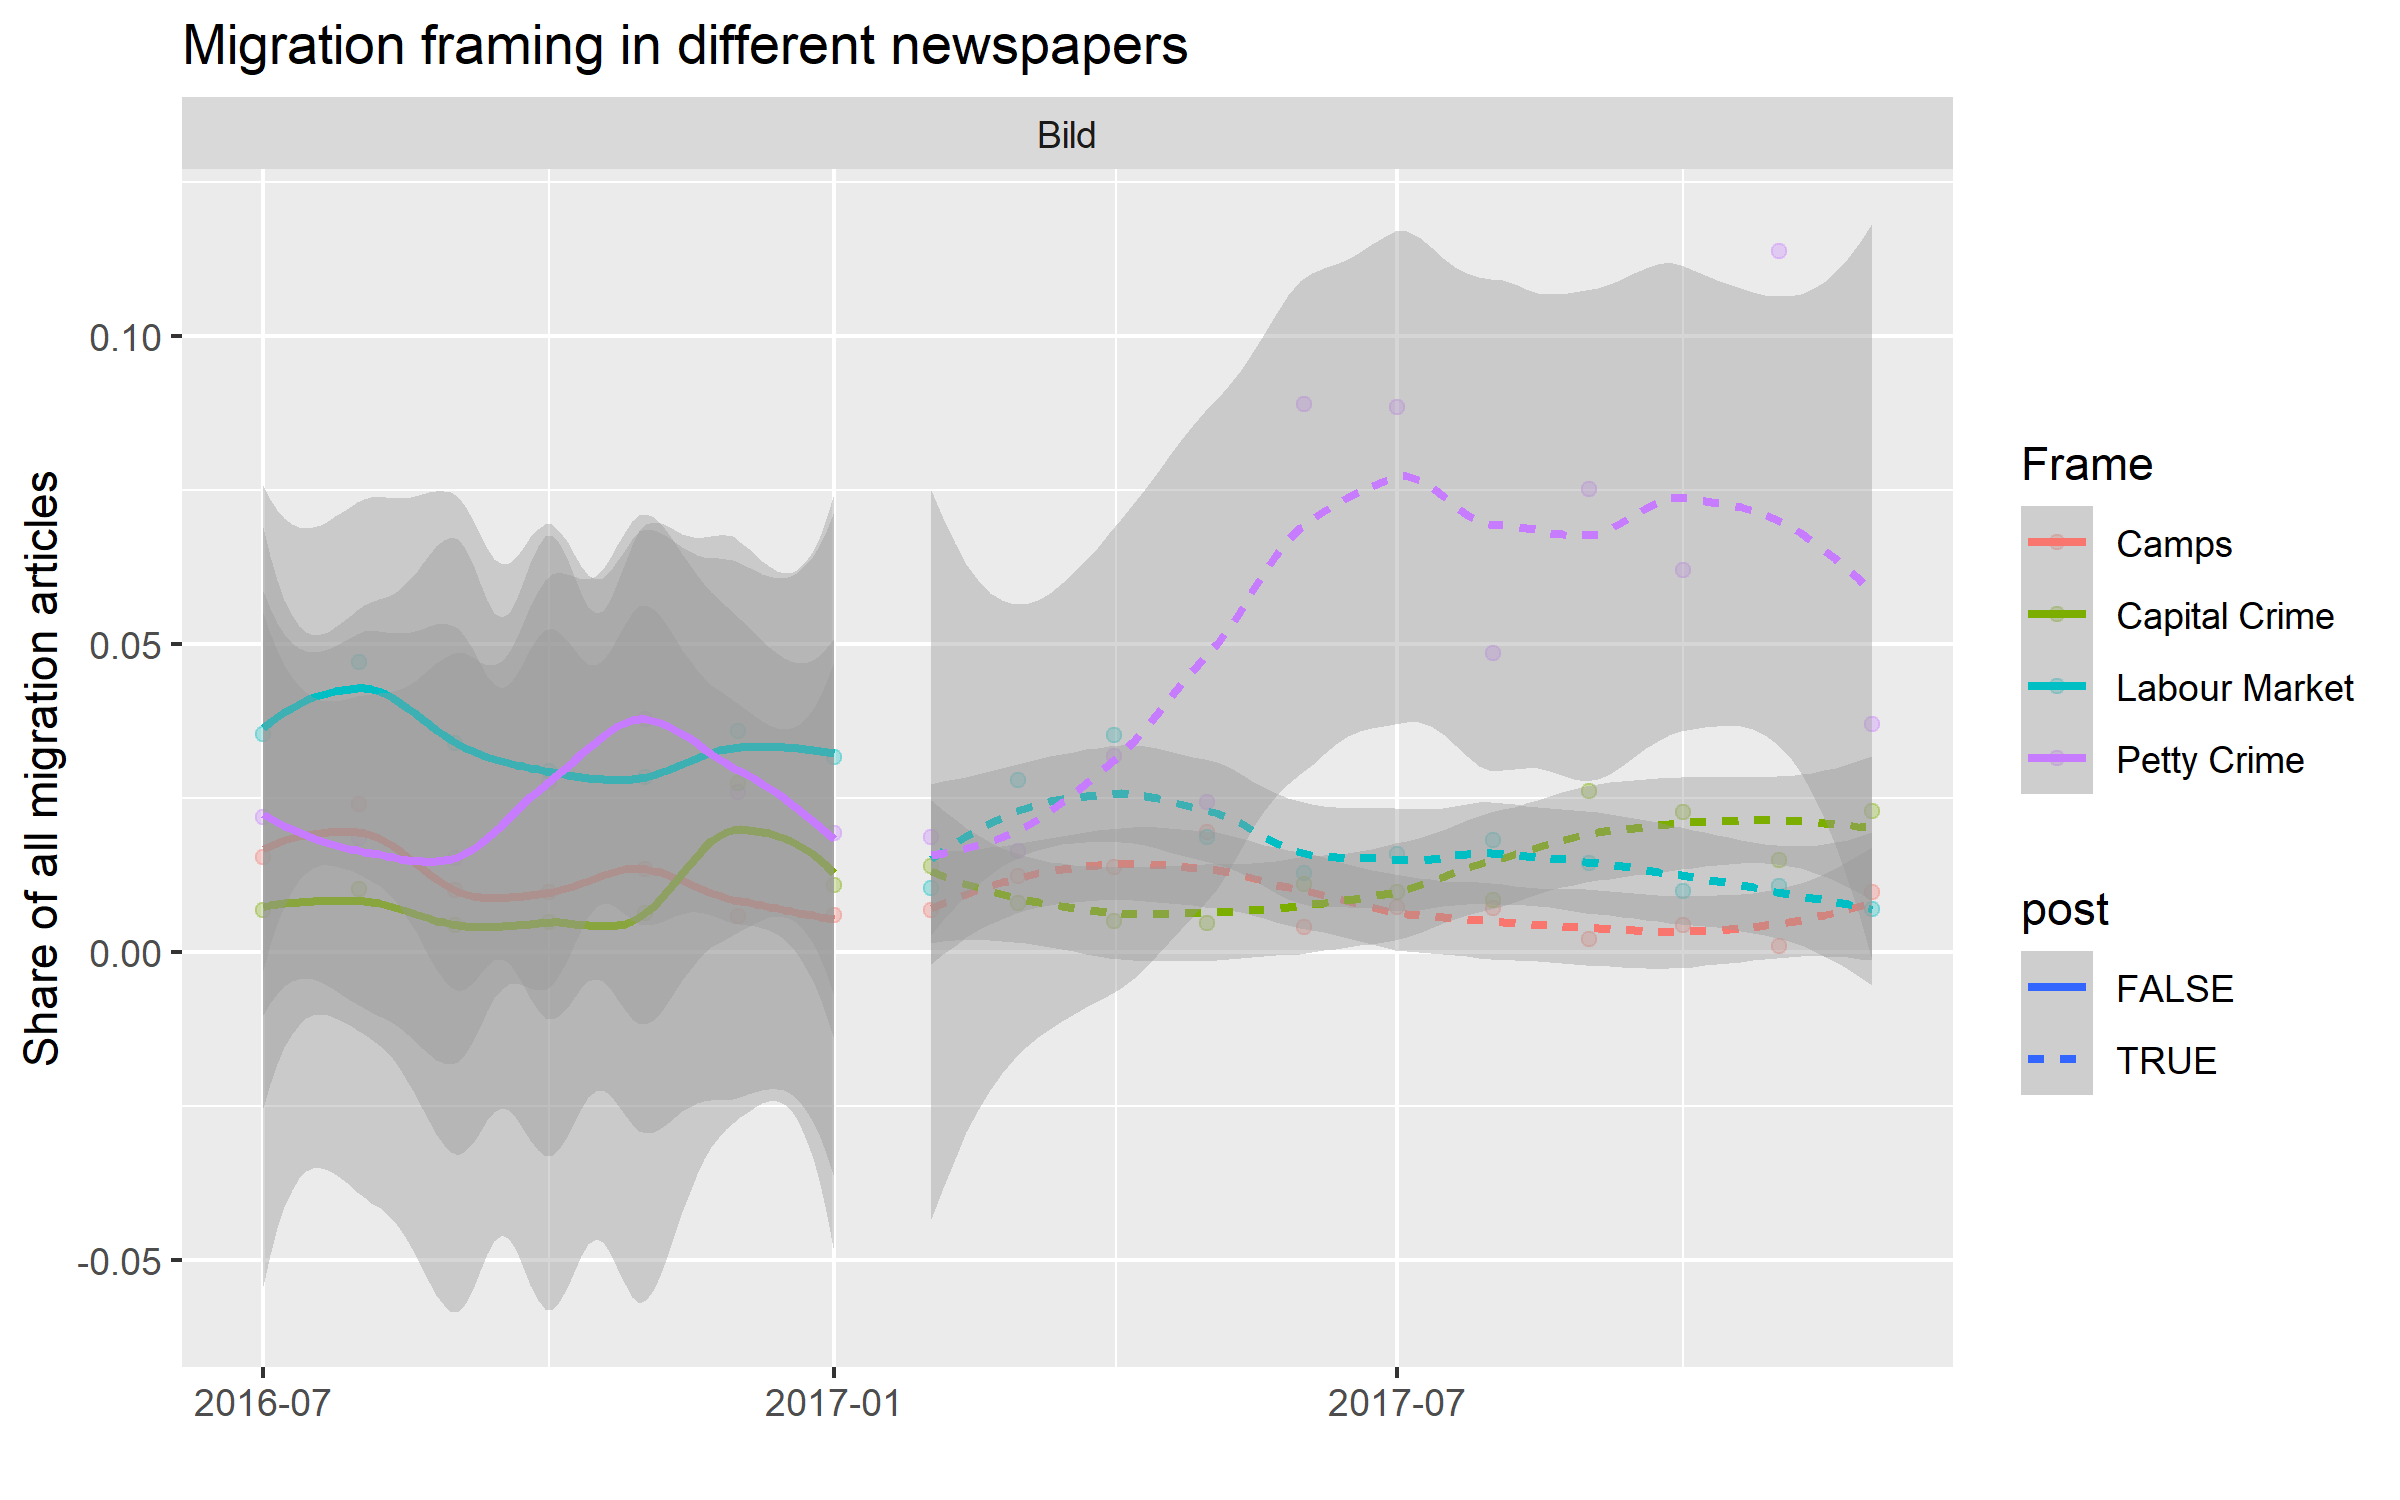
\includegraphics{vis/frames_papers_focus_pres.png}
\end{frame}

\begin{frame}{Specifications DiD}
\protect\hypertarget{specifications-did}{}
\centering

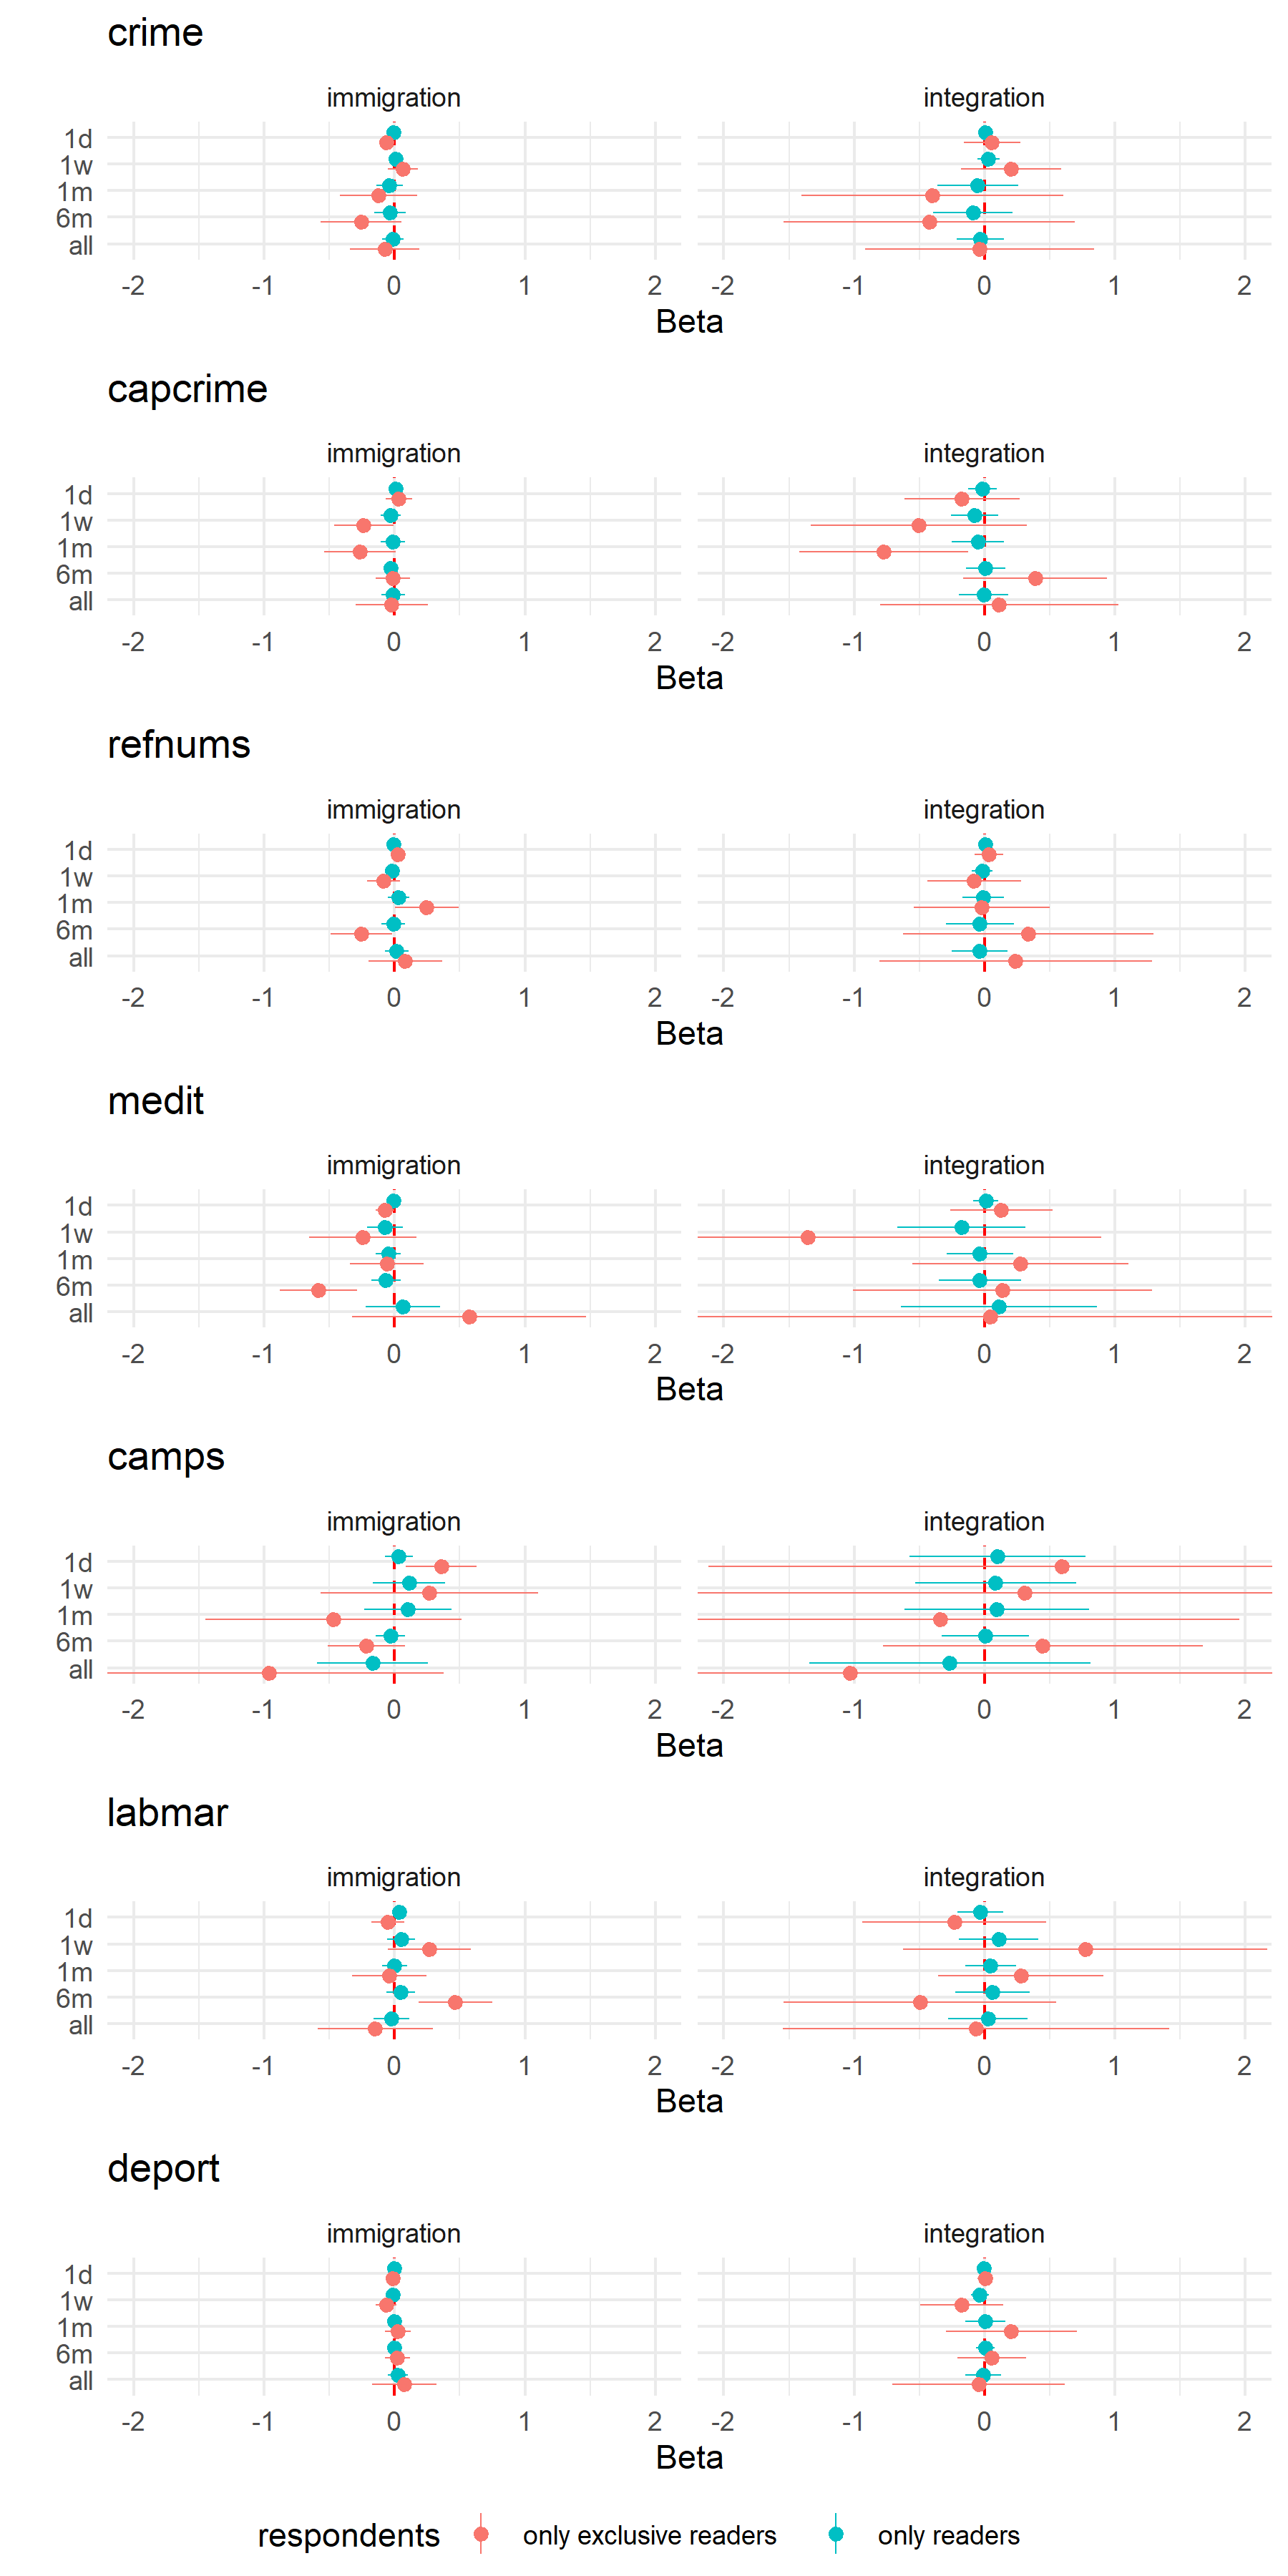
\includegraphics[width=0.7\textwidth,height=\textheight]{vis/effectplot_frames_did.png}
\end{frame}

\begin{frame}{Specifications 2-way FE}
\protect\hypertarget{specifications-2-way-fe}{}
\centering

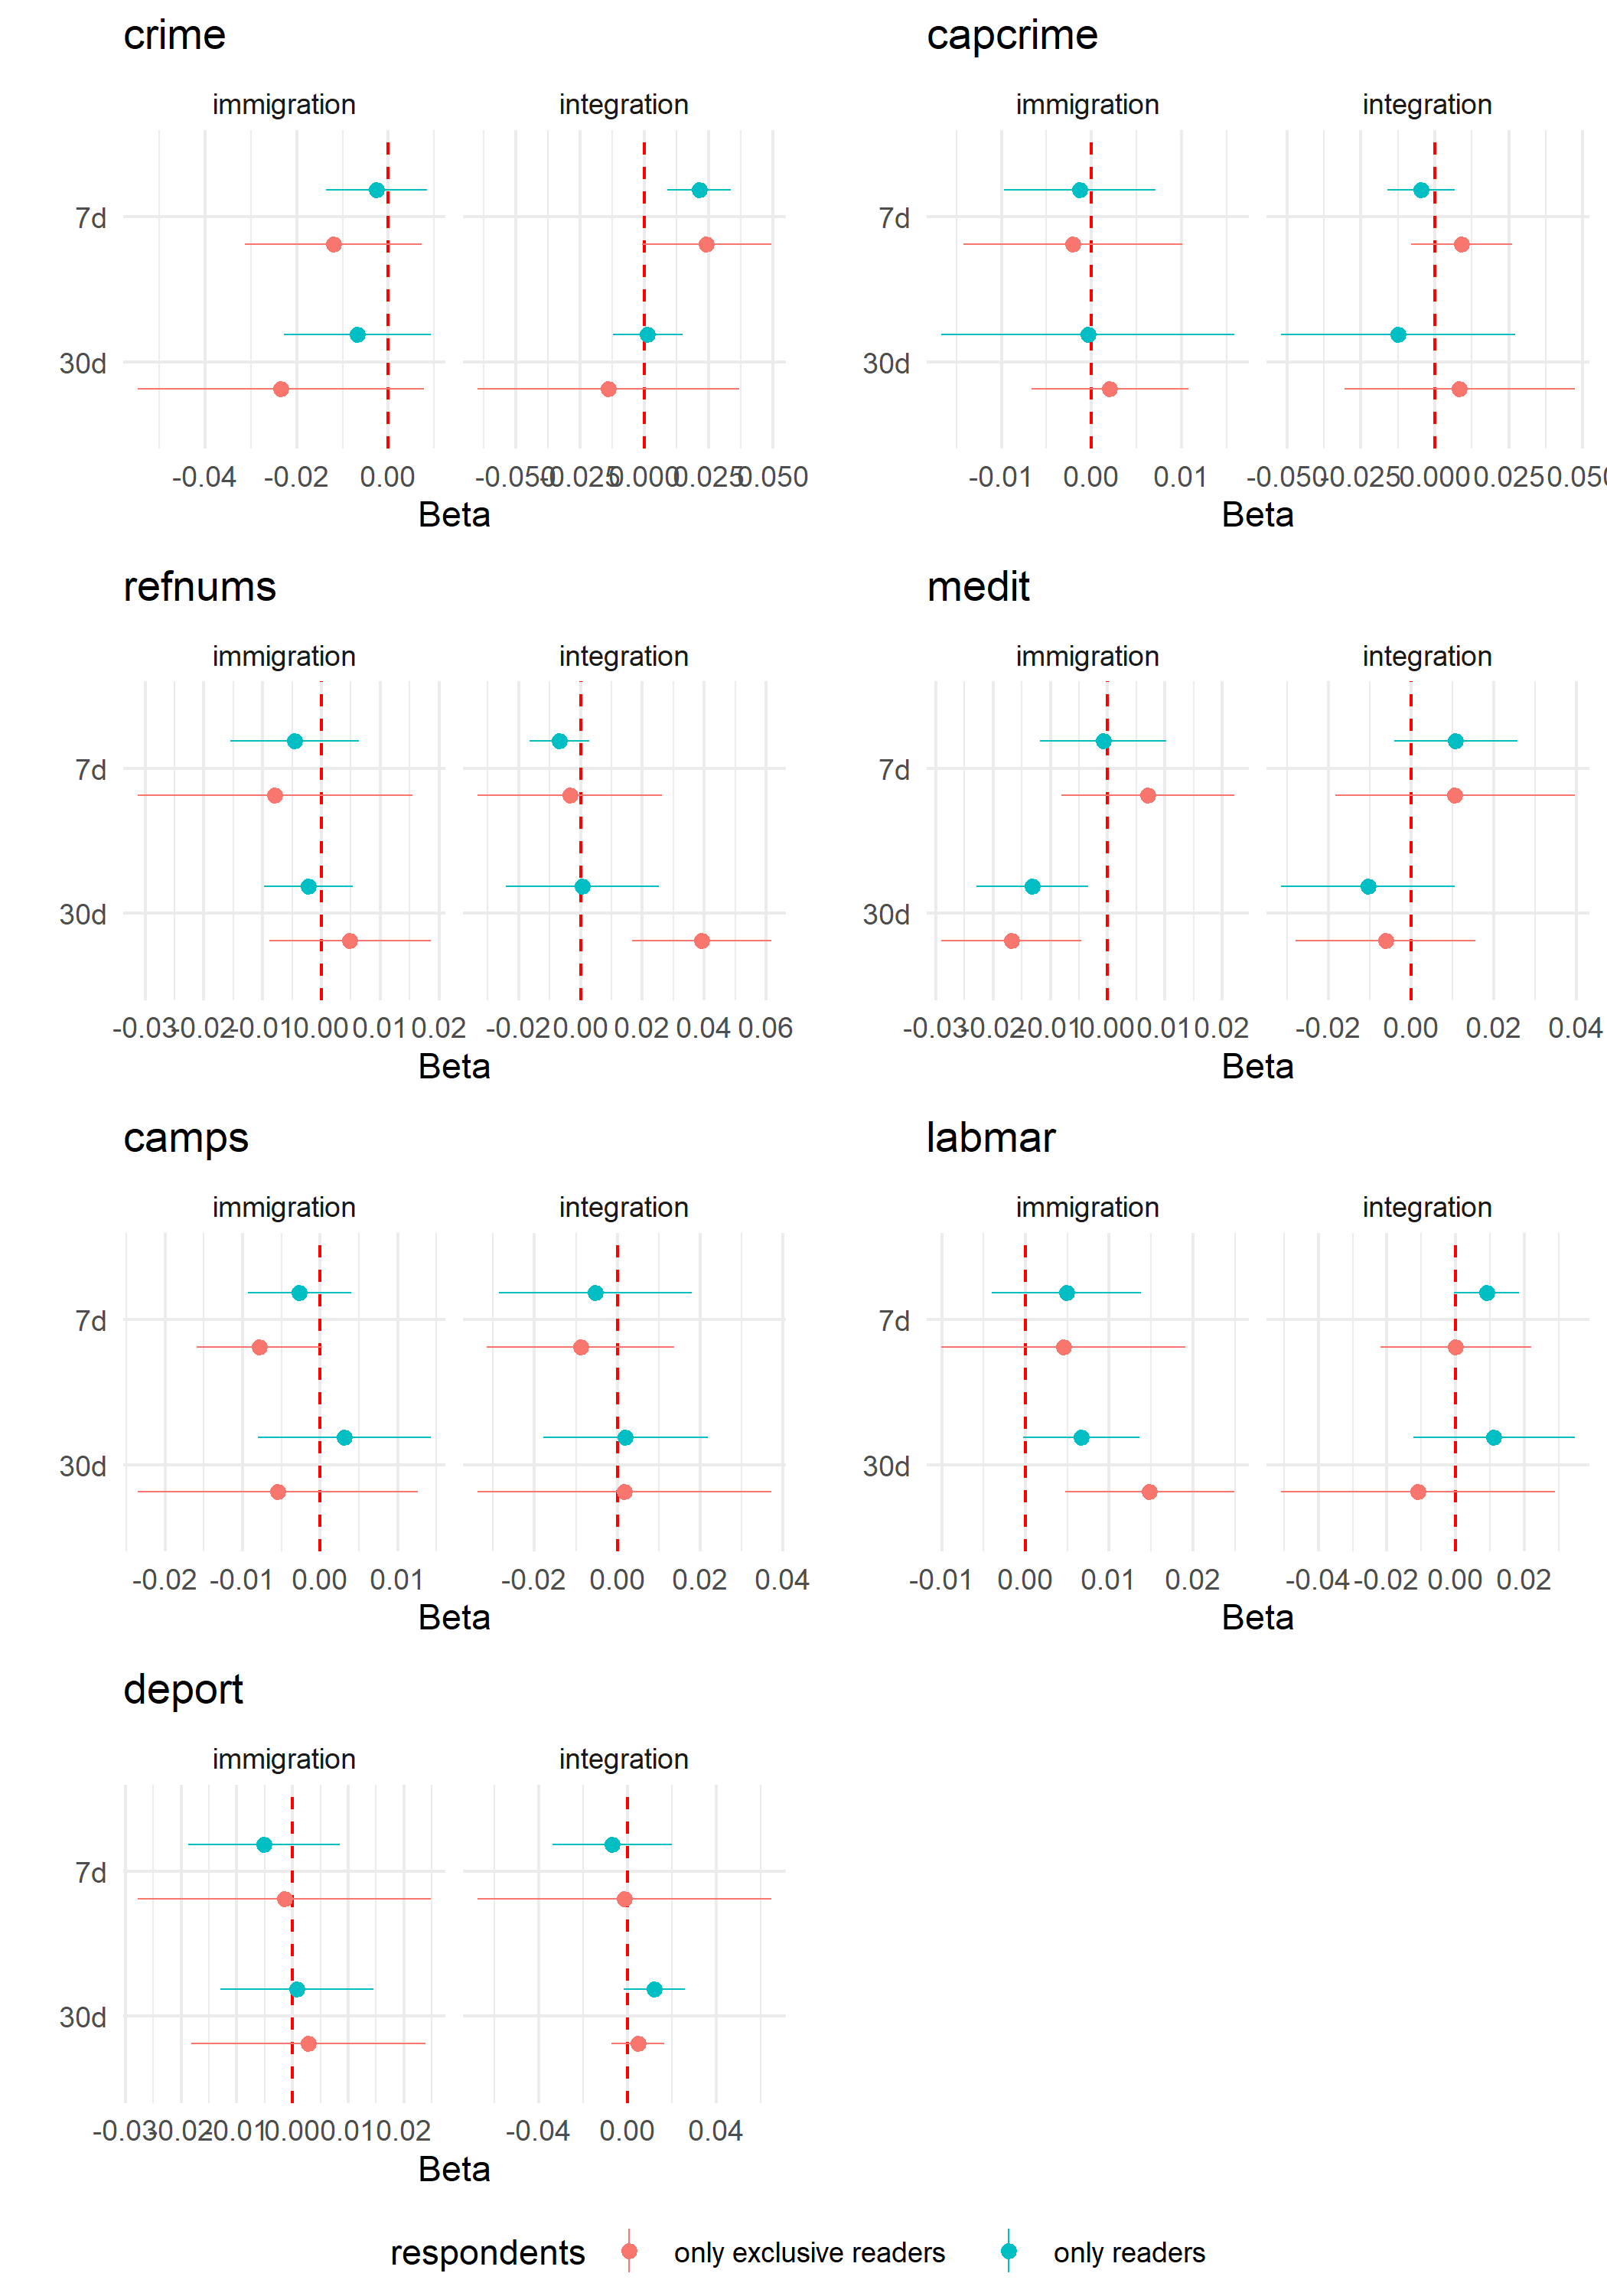
\includegraphics[width=0.7\textwidth,height=\textheight]{vis/effectplot_frames_fe_abs.png}
\end{frame}

\hypertarget{resources}{%
\section{Resources}\label{resources}}

\begin{frame}[allowframebreaks]{Resources}
\protect\hypertarget{resources-1}{}
\hypertarget{refs}{}
\begin{CSLReferences}{1}{0}
\leavevmode\hypertarget{ref-Ajzen2000}{}%
Ajzen, Icek, and Martin Fishbein. 2000. {``{Attitudes and the
Attitude-Behavior Relation: Reasoned and Automatic Processes}.''}
\emph{European Review of Social Psychology} 11 (1): 1--33.
\url{https://doi.org/10.1080/14792779943000116}.

\leavevmode\hypertarget{ref-Arceneaux2013}{}%
Arceneaux, Kevin, and Martin Johnson. 2013. \emph{{Changing Mind or
Changing Channels? Partisan News in an Age of Choice}}. University of
Chicago Press.

\leavevmode\hypertarget{ref-Baum2008}{}%
Baum, Matthew A., and Phil Gussin. 2008. {``{In the Eye of the Beholder:
How Information Shortcuts Shape Individual Perceptions of Bias in the
Media}.''} \emph{Quarterly Journal of Political Science} 3 (1): 1--31.
https://doi.org/\url{http://dx.doi.org/10.1561/100.00007010}.

\leavevmode\hypertarget{ref-Bennett2008}{}%
Bennett, W. Lance, and Shanto Iyengar. 2008. {``{A new era of minimal
effects? The changing foundations of political communication}.''}
\emph{Journal of Communication} 58 (4): 707--31.
\url{https://doi.org/10.1111/j.1460-2466.2008.00410.x}.

\leavevmode\hypertarget{ref-Boomgaarden2009}{}%
Boomgaarden, Hajo G., and Rens Vliegenthart. 2009. {``{How news content
influences anti-immigration attitudes: Germany, 1993-2005}.''}
\emph{European Journal of Political Research} 48 (4): 516--42.
\url{https://doi.org/10.1111/j.1475-6765.2009.01831.x}.

\leavevmode\hypertarget{ref-Busby2019}{}%
Busby, Ethan, D. J. Flynn, and James N. Druckman. 2019. {``{Studying
Framing Effects on Political Preferences}.''} \emph{Doing News Framing
Analysis II}, 27--50. \url{https://doi.org/10.4324/9781315642239-2}.

\leavevmode\hypertarget{ref-Chiang2011a}{}%
Chiang, Chun Fang, and Brian Knight. 2011. {``{Media bias and influence:
Evidence from newspaper endorsements}.''} \emph{Review of Economic
Studies} 78 (3): 795--820. \url{https://doi.org/10.1093/restud/rdq037}.

\leavevmode\hypertarget{ref-Converse1962}{}%
Converse, Philip E. 1962. {``{Information flow and the stability of
partisan attitudes}.''} \emph{Public Opinion Quarterly} 26 (4): 578--99.
\url{https://doi.org/10.1086/267129}.

\leavevmode\hypertarget{ref-Durante2012}{}%
Durante, Ruben, and Brian Knight. 2012. {``{Partisan control, media
bias, and viewer responses: Evidence from berlusconi's italy}.''}
\emph{Journal of the European Economic Association} 10 (3): 451--81.
\url{https://doi.org/10.1111/j.1542-4774.2011.01060.x}.

\leavevmode\hypertarget{ref-Foos2020}{}%
Foos, Florian, and Daniel Bischof. 2020. {``{Can the tabloid media
create Eurosceptic attitudes? A quasi-experiment on media innuence in
England},''} no. page 26.

\leavevmode\hypertarget{ref-Gentzkow2011}{}%
Gentzkow, Matthew, Jesse M. Shapiro, and Michael Sinkinson. 2011.
{``{The effect of newspaper entry and exit on electoral politics}.''}
\emph{American Economic Review} 101 (7): 2980--3018.
\url{https://doi.org/10.1257/aer.101.7.2980}.

\leavevmode\hypertarget{ref-GLES2019LongTermTracking}{}%
GLES. 2019. {``{Longterm-Online-Tracking 2009-2017 (GLES)}.''} Cologne:
GESIS Data Archive.
https://doi.org/\url{https://doi.org/10.4232/1.13416}.

\leavevmode\hypertarget{ref-Guess2021}{}%
Guess, Andrew M, Pablo Barberá, Simon Munzert, and Junghwan Yang. 2021.
{``{The consequences of online partisan media},''} 1--8.
\url{https://doi.org/10.1073/pnas.2013464118/-/DCSupplemental.y}.

\leavevmode\hypertarget{ref-Leeper2020}{}%
Leeper, Thomas J., and Rune Slothuus. 2020. {``{How the News Media
Persuades}.''} \emph{The Oxford Handbook of Electoral Persuasion},
150--68. \url{https://doi.org/10.1093/oxfordhb/9780190860806.013.4}.

\leavevmode\hypertarget{ref-McCombs1972}{}%
McCombs, Maxwell E., and Donald L Shaw. 1972. {``{The agenda-setting
function of mass media}.''} \emph{Public Opinion Quarterly} 36 (2):
176--87.

\leavevmode\hypertarget{ref-Nelson1997}{}%
Nelson, Thomas E, Rosalee A Clawson, and Zoe Oxley. 1997. {``{Media
Framing of a Civil Liberties Conflict and Its Effect on Tolerance}.''}
\emph{American Political Science Review} 91 (3): 567--83.

\leavevmode\hypertarget{ref-Roberts2014}{}%
Roberts, Margaret E., Brandon M. Stewart, Dustin Tingley, Christopher
Lucas, Jetson Leder-Luis, Shana Kushner Gadarian, Bethany Albertson, and
David G. Rand. 2014. {``{Structural topic models for open-ended survey
responses}.''} \emph{American Journal of Political Science} 58 (4):
1064--82. \url{https://doi.org/10.1111/ajps.12103}.

\leavevmode\hypertarget{ref-Spirig2020}{}%
Spirig, Judith. 2020. {``{Media Take-Over and Voting Behavior : Can
Politician-Owned Newspapers Sway Voters ?}''}

\leavevmode\hypertarget{ref-Stetka2020}{}%
Štětka, Václav, Sabina Mihelj, and Fanni Tóth. 2020. {``{The Impact of
News Consumption on Anti-immigration Attitudes and Populist Party
Support in a Changing Media Ecology}.''} \emph{Political Communication}
38 (5): 539--60. \url{https://doi.org/10.1080/10584609.2020.1820647}.

\leavevmode\hypertarget{ref-Taber2006}{}%
Taber, Charles S, and Milton Lodge. 2006. {``{Motivated Skepticism in
the Evaluation of Political Beliefs}.''} \emph{American Journal of
Political Science} 50 (3): 755--69.

\leavevmode\hypertarget{ref-Zaller1992}{}%
Zaller, John. 1992. \emph{{The nature and origins of mass opinion}}.
Cambridge University Press.

\end{CSLReferences}
\end{frame}

\end{document}
